% Chapter 1

\chapter{Photoionization of Co$^{+}$ and electron-impact excitation of Co$^{2+}$} 
% Main chapter title
\label{cha:cobalt} 
% For referencing the chapter elsewhere, use \ref{Chapter1} 
\lhead{Chapter 7. \emph{Transitions involving ions of cobalt}} 
% This is for the header on each page - perhaps a shortened title

%----------------------------------------------------------------------------------------

\section{Introduction}\label{sec:co_introduction}
Lowly ionized species of cobalt are often observed in astrophysical objects such as supernovae (SNe), cool stars \citep{2010MNRAS.401.1334B}, early type stars \citep{1993A&A...274..335S} and the solar spectrum \citep{1998ApJS..117..261P}. These applications necessitate the need for high quality atomic data which accurately describe the processes of excitation and photoionization. This is further evidenced in SNe by following the nucleosynthesis decay path of $^{56}$Ni$\rightarrow ^{56}$Co$\rightarrow ^{56}$Fe, which occurs post explosion. The principal aim is to facilitate modelling within the astrophysics community with accurate and up-to-date atomic transitions necessary for synthetic spectral analysis, allowing detailed comparisons to be carried out with observation. Stand alone reports stress both the importance and absence of photon/electron interaction with systems of iron, cobalt and nickel \citep{1995ASPC...78..291R, 2011Ap&SS.336...87H, 2014MNRAS.441.3249D}. 

The Opacity Project has been an invaluable source for such data, but is often limited when considering iron peak species. These important Fe-peaks are difficult to investigate due to their open d-shell structure which gives rise to many hundreds of target states for each electronic configuration and typically thousands of closely coupled channels. Hence the target states require substantial configuration-interaction expansions for their accurate representation. Fe$^{+}$ is one such challenging case where over the last decade calculations for this ion have grown in size, complexity and sophistication. Significant differences, however, are still observed in the resulting atomic data as can be seen by the latest two major evaluations for the electron-impact excitation of Fe$^{+}$ \citep{2007A&A...475..765R, 2015ApJ...808..174B}. Factors of 2 - 3 disparity being the norm at the temperature of maximum abundance 10,000 K for many of the low-lying forbidden lines.

There have been a number of studies focused on essential atomic data between species of Co - Co$^{2+}$concerning bound transitions. These include oscillator strengths for neutral cobalt between 2276\AA - 9357\AA ~\citep{1982ApJ...260..395C}, transition probabilities through a multi configuration approach for comparison with observed infrared spectra \citep{1988A&A...200L..25N}, and also a relativistic Hartree-Fock approach between the lowest 47 levels of Co$^{+}$ \citep{1998A&AS..129..147Q}. More recently, collision strengths and other radiative data have been calculated for Co$^{+}$ \citep{2016MNRAS.456.1974S} and Co$^{3+}$ \citep{2016ADNDT.107..140A}. During the preparation of this work, it has come to our attention a detailed study of electron-impact excitation cross-sections for Co$^{2+}$ conducted by \citet{2016MNRAS.tmp..556S}.

The early ion stages of, and even neutral cobalt are clearly important as detailed in the literature. Early observations have shown strong Co {\sc ii} lines in $\eta$ Carinae \citep{1976MNRAS.174P..59T}, confirmed more recently by \citet{2001AJ....122..322Z} to be unusually strong, and in the UV regime in $\zeta$ Oph \citep{1979ApJ...234..506S}, confirmed by \citet{1993ApJ...413L..51F}. These lines are apparent in the binary star HR5049 \citep{1980A&A....85..138D, 1982Obs...102..138D} - which previously have been unidentified due to the lack of laboratory data. In this same study, the amount of cobalt is estimated to be around 3 orders of magnitude overabundant relative to the Sun.

Due to the decay path of $^{56}$Ni, cobalt is often observed in various SNe at both early and late epochs. The Type II SNe 1987A, exploded in the large magellanic cloud, providing a study of the expanding ejecta as the $^{56}$Co decays. A large proportion of Fe {\sc ii} and Co {\sc ii} lines are blended due to their similar ionization energies, but the strong 1.547$\mu$m line occurs from the transition a$^5$F$_5\rightarrow$ b$^3$F$_4$ \citep{1989MNRAS.238..193M, 1993ApJ...419..824L} in Co {\sc ii}. The Co {\sc iii} a$^4$F$_{9/2}\rightarrow$ a$^2$G$_{9/2}$ 0.589$\mu$m line in another Type II SNe, 1991bg, is used as a diagnostic to infer the mass of synthesized $^{56}$Ni. It is also possible to deduce important properties such as the mass of the exploding star \citep{1997MNRAS.284..151M}.

The Co$^{+}$ and Co$^{2+}$ ions under discussion in this Chapter have also received much interest over the last decade. The mid infrared spectrum of SNe 2003hv and 2005df show strong Co {\sc iii} line emissions and even emission from Co {\sc iv} \citep{2007ApJ...661..995G}. However, the collisional processes included in the model have been approximated using statistically weighted collision strengths. A study of the near infrared spectra from SNe 2005df yields strong Co {\sc iii} emission lines initially but by day 200 the majority of cobalt has expectedly decayed down to Fe \citep{2015ApJ...806..107D}. A number of Co {\sc iii} lines are still visible at late times for Type Ia SNe as documented in \citep{1995ASPC...78..291R}. These lines would be extremely beneficial in particular diagnostic work, but as outlined above, little collisional data exists. In addition the photoionization cross-sections employed in the models are obtained from a central potential approximation \citep{1979ApJS...40..815R} for the ground state only. Co {\sc iii} is also present in SNe 2014J and the 11.888$\mu$m line is useful for monitoring the time evolution of the photosphere, and again, the mass of synthesized Ni \citep{2015ApJ...798...93T}. It is evident from these works and the associated applications the importance of conducting sophisticated and complete calculations for the lowly ionized Fe-peak species of Fe, Ni and Co.

In Section \ref{sec:co_structure} we discuss the development of an accurate structure model for Co$^{2+}$ to include in the $R$-matrix collisional calculations for electron-impact excitation and photoionization. The accuracy of this model will be tested by reassessing energy levels of the target states and the conformity of transition probabilities with previous assessments. In Section \ref{sec:co_results} we present level-resolved ground and excited state photoionization cross-sections for Co$^{+}$ and a selection of collision strengths and effective collision strengths for the electron impact excitation of Co$^{2+}$. Comparisons will be made where possible with existing data but these are limited. Finally we summarise our findings and conclusions in Section \ref{sec:co_conclusions}.
%__________________________________________________________________
\section{Important transitions for synthetic spectral\\ modelling}\label{sec:co_structure}
This work focuses initially on transitions that occur between discrete states of our atomic system, Co$^{2+}$. In Figure \ref{fig:co_transitions} we graphically present some of the most important lines in the infrared and visible energy bands of the spectrum. Transitions among the ground state term $^4$F and levels of the parent ion Co$^{2+}$ with configuration 3d$^7$ are shown on the right hand side. The neighbouring system Co$^{+}$ is also shown on the left complete with its fine-structure split $J$ levels to indicate the photoionization process under investigation. 


%
%%
%%%
%%%%
\begin{figure}[h]
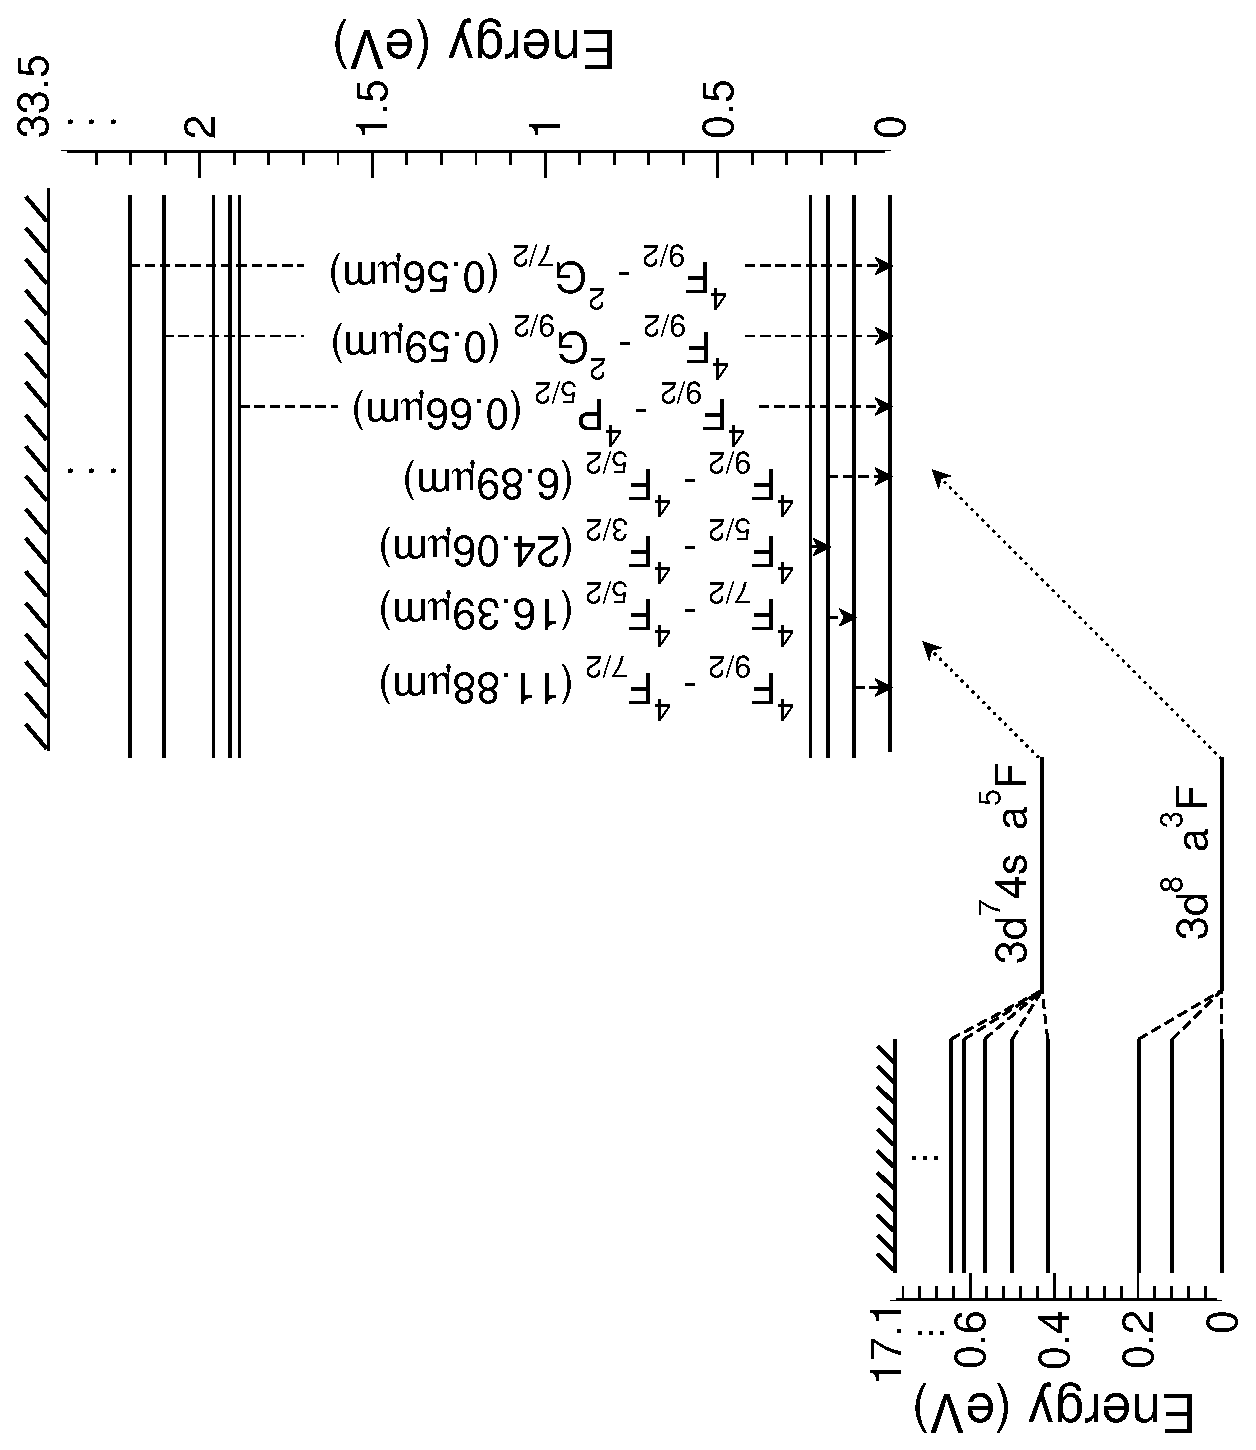
\includegraphics[scale=0.59, angle=-90]{Figures/Cobalt/figure1.eps}
\caption{Important lines in the infrared and visible energy bands between levels of Co$^{2+}$ amongst the 3d$^7$ configuration and involving the ground term $^4$F. The neighbouring system of Co$^{+}$ is to the left with its split $J\pi$ levels to indicate the photoionization process. \label{fig:co_transitions}}
\end{figure}
%%%%
%%%
%%
%


\subsection{Target description and bound state transitions}\label{sec:co_target}
We first detail results obtained from transitions within the bound system of Co$^{2+}$ and our {\it ab initio} energy eigenvalues. The Dirac-Coulomb Hamiltonian from equation (\ref{eq:many_dirac_ham}) is then incorporated into the {\sc grasp}0 computer package, with $Z=27$ as the atomic number and $N=25$ as the number of electrons for the system.

As stated in Section \ref{sec:co_introduction}, partially filled d-shell systems are difficult due to the hundreds of levels associated with a single configuration. Initially, we include three configurations, 3d$^7$ and 3d$^6$[4s, 4p] during the optimization process, denoted as \textit{model 1}, which results in a total of 262 fine-structure levels to describe the Co$^{2+}$ ion. The ground state of which is 3d$^7$a$^4$F$_{9/2}$. Next we optimize all orbitals up to $3d$ on the configurations from the double electron promotions, 3s$^2$, 3p$^2$ $\rightarrow$ 3d$^2$ and include in the total calculation all configurations from \textit{model 1} plus 3p$^6$3d$^9$ (double promotion from $3s$ to $3d$) and 3s$^2$3p$^4$3d$^9$ (double promotion from $3p$ to $3d$). This technique can be useful as it alleviates the necessity to include numerous pseudo states into the calculation. We denote this \textit{model 2} which constitutes a total of 292 levels. Finally, by including 3d$^5$[4s$^2$, 4p$^2$] and 3d$^5$4s4p, the number of levels drastically increases to 1,259 levels, and we label this as \textit{model 3}. 

We present in Table \ref{tab:co_energy} our {\it ab initio} energy levels obtained from {\sc grasp}0 in eV for the lowest lying 38 levels alongside those observed by \citet{1985aeli.book.....S}. This work is a compilation of observed spectra in the 650\AA - 3800\AA ~wavelength range. We also present the $\%$ difference between \citet{1985aeli.book.....S} and our \textit{model 2}, and also provide the lowest 15 levels of \citet{2016MNRAS.tmp..556S}. Good agreement is found ($<$10\% for the majority of levels) between the present \textit{model 2} and \textit{model 3} energies and those of \citet{2016MNRAS.tmp..556S}. As with other Fe-peak ions, the energy levels of the lowest-lying 3d$^{7}$ fine-structure states are notoriously difficult to determine. The highest disparities are found for these levels when compared with \citet{1985aeli.book.....S}, the largest being for the 3d$^{7}$ $^{4}$F$_{9/2}$ $\rightarrow$ 3d$^{7}$ $^{2}$H$_{11/2}$ (1-12) transition. For levels indexed above 17 the differences are at most 10-11$\%$ and for many levels by considerably less. The main problem is due to the fact that a single $3d$ orbital is used to describe the configuration state functions for multiple configurations of type 3d$^{7}$ and 3d$^{6}$4s. Similar differences were reported by \citet{2009ADNDT..95..910R} for the low-lying 3d$^{7}$ fine-structure levels of Fe$^+$. 

%
%%
%%%
%%%%
\begin{table*}[h]
\footnotesize
\begin{center}
\begin{tabular}{@{} l *8c @{}}
            \hline
\multicolumn{1}{c}{Index} & Level & \textit{S\&C} & \textit{model 1}  & \textit{model 2} & $\%$ & \textit{model 3} & \textit{Storey} \\
            \hline
\multicolumn{1}{c}{  1} & 3d$^7$ a$^4$F$_{ 9/2}$ &  0.00000  & 0.00000  & 0.00000 & 0.0 & 0.00000  & 0.00000\\
\multicolumn{1}{c}{  2} & 3d$^7$ a$^4$F$_{ 7/2}$ &  0.10430  & 0.10355  & 0.09939 & 4.7 & 0.09980    & 0.10216\\
\multicolumn{1}{c}{  3} & 3d$^7$ a$^4$F$_{ 5/2}$ &  0.17994  & 0.18001  & 0.17255 &  4.1 & 0.17321   & 0.17705\\
\multicolumn{1}{c}{  4} & 3d$^7$ a$^4$F$_{ 3/2}$ &  0.23145  & 0.23263  & 0.22280 &  3.7 & 0.22362  & 0.22838 \\
\multicolumn{1}{c}{  5} & 3d$^7$ a$^4$P$_{ 5/2}$ &  1.88480  &  2.39405  & 2.20436 &  16.9 & 2.19761   &  2.29369\\
\multicolumn{1}{c}{  6} & 3d$^7$ a$^4$P$_{ 3/2}$ &  1.91285  & 2.42637  & 2.23271 &   16.7 & 2.22608   & 2.32904\\
\multicolumn{1}{c}{  7} & 3d$^7$ a$^4$P$_{ 1/2}$ &  1.96036  & 2.47283 & 2.27875 &   16.2 & 2.27244   &   2.37033\\
\multicolumn{1}{c}{  8} & 3d$^7$ a$^2$G$_{ 9/2}$ &  2.10496  & 2.39059  & 2.38992 &  13.5 & 2.38842   & 2.42773\\
\multicolumn{1}{c}{  9} & 3d$^7$ a$^2$G$_{ 7/2}$ &  2.20273  & 2.48967  & 2.48250 &   12.7 & 2.48138 & 2.52395 \\
\multicolumn{1}{c}{ 10} & 3d$^7$ a$^2$P$_{ 3/2}$ &  2.50385   & 3.16229 &     2.85243 &   13.9 & 2.84334   & 3.17809\\
\multicolumn{1}{c}{ 11} & 3d$^7$ a$^2$P$_{ 1/2}$ &  2.59356  & 3.27065 &    2.96428 & 14.3 & 2.95673    & 3.28236 \\
\multicolumn{1}{c}{ 12} & 3d$^7$ a$^2$H$_{11/2}$ &  2.81696  & 3.18356 &    3.35270 & 19.0 & 3.35260    & 3.18478\\
\multicolumn{1}{c}{ 13} & 3d$^7$ a$^2$H$_{ 9/2}$ &  2.90548  &  3.26836 &     3.43116 &  18.1 & 3.43143  & 3.27058\\
\multicolumn{1}{c}{ 14} & 3d$^7$ a$^2_2$D$_{5/2}$ &  2.85893  & 3.44672 &    3.06277 &  7.1 & 3.04740   & 3.44726\\
\multicolumn{1}{c}{ 15} & 3d$^7$ a$^2_2$D$_{ 3/2}$ &  3.00498  & 3.60358 &    3.23140 & 7.5 & 3.21873   &  3.59963 \\
\multicolumn{1}{c}{ 16} & 3d$^7$ a$^2$F$_{ 5/2}$ &  4.59002  &  5.51392 &    5.36609 &  16.9 & 5.35716   & - \\
\multicolumn{1}{c}{ 17} & 3d$^7$ a$^2$F$_{ 7/2}$ &  4.62666  &  5.55837 &    5.40863 &   16.9 & 5.39998  & - \\
\multicolumn{1}{c}{ 18} & 3d$^6$4s a$^6$D$_{ 9/2}$ &  5.75762  & 6.70846 &     6.06849 & 5.4 & 6.20178   & - \\
\multicolumn{1}{c}{ 19} & 3d$^6$4s a$^6$D$_{ 7/2}$ &  5.82764  &  6.78942 &     6.14650 &  5.5 & 6.27925 & -  \\
\multicolumn{1}{c}{ 20} & 3d$^6$4s a$^6$D$_{ 5/2}$ &  5.87876  &  6.84869 &    6.20378 & 5.5 & 6.33614   & - \\
\multicolumn{1}{c}{ 21} & 3d$^6$4s a$^6$D$_{ 3/2}$ &  5.91387  & 6.88947 &    6.24324 &  5.5 & 6.37536 & - \\ 
\multicolumn{1}{c}{ 22} & 3d$^6$4s a$^6$D$_{ 1/2}$ &  5.93448  & 6.91340 &    6.26643 &  5.6 & 6.39840 & - \\
\multicolumn{1}{c}{ 23} & 3d$^6$4s a$^4$D$_{ 7/2}$ &  6.90954  & 8.42015 &    7.72255 &  11.8 & 8.04998   & - \\
\multicolumn{1}{c}{ 24} & 3d$^6$4s a$^4$D$_{ 5/2}$ &  6.98946  &  8.51285 &    7.81196 &   11.8 & 8.13868& - \\
\multicolumn{1}{c}{ 25} & 3d$^6$4s a$^4$D$_{ 3/2}$ &  7.04166  &  8.57368 &    7.87084 &  11.8 & 8.19722 & - \\
\multicolumn{1}{c}{ 26} & 3d$^6$4s a$^4$D$_{ 1/2}$ &  7.07167  &  8.60877 &    7.90480 &  11.8 & 8.23095 & - \\
\multicolumn{1}{c}{ 27} & 3d$^7$ a$^2_1$D$_{ 3/2}$ &  -  &  8.67161 & 7.93064 &   - & 7.96545 & - \\
\multicolumn{1}{c}{ 28} & 3d$^7$ a$^2_1$D$_{ 5/2}$ &  -  & 8.61018 &  8.00119 & - & 7.89375 & - \\
\multicolumn{1}{c}{ 29} & 3d$^6$4s b$^4$P$_{ 5/2}$ &  8.79471  &  10.25065 &   9.63834 &  9.6 & 9.80974  &   - \\
\multicolumn{1}{c}{ 30} & 3d$^6$4s a$^4$H$_{13/2}$ &  8.88014  &  10.00120 &    9.38243 &  5.6 & 9.55349  & - \\
\multicolumn{1}{c}{ 31} & 3d$^6$4s a$^4$H$_{11/2}$ &  8.91121  & 10.03198  &    9.41243 &  5.6 & 9.58337  & - \\
\multicolumn{1}{c}{ 32} & 3d$^6$4s a$^4$H$_{ 9/2}$ &  8.93719  &  10.05805 &    9.43786 &  5.6 & 9.60883   & - \\
\multicolumn{1}{c}{ 33} & 3d$^6$4s a$^4$H$_{ 7/2}$ &  8.96040  &  10.08057 &    9.45963 &  5.6 & 9.63075   & - \\
\multicolumn{1}{c}{ 34} & 3d$^6$4s b$^4$P$_{ 3/2}$ &  8.96926  &  10.46563 &   9.84580 &  9.8 & 10.01710   & - \\
\multicolumn{1}{c}{ 35} & 3d$^6$4s b$^4$P$_{ 1/2}$ &  9.07744  &  10.59439 &    9.97061 &  9.8 & 10.14009  & - \\
\multicolumn{1}{c}{ 36} & 3d$^6$4s b$^4$F$_{ 9/2}$ &  9.08631  &  10.42302 &    9.81043 &  8.0 & 9.98184  & - \\
\multicolumn{1}{c}{ 37} & 3d$^6$4s b$^4$F$_{ 7/2}$ &  9.11782  &  10.46016 &    9.84605 &  8.0 & 10.01692  & - \\
\multicolumn{1}{c}{ 38} & 3d$^6$4s b$^4$F$_{ 5/2}$ &  9.14093  &  10.49101 &    9.87566 &  8.0 & 10.04624  & - \\
            \bottomrule
 \end{tabular}
 \caption{Energies for the lowest 38 levels of Co$^{2+}$ are presented in eV relative to the ground state 3d$^7$ a$^4$F$_{9/2}$. \textit{S\&C} is from the work of \citet{1985aeli.book.....S}. \textit{model 1}, \textit{model 2}, \textit{model 3} are the current results from {\sc grasp}0 and the last column are the lowest 15 levels from \citet{2016MNRAS.tmp..556S}. We also present the $\%$ difference between our current \textit{model 2} and \textit{S\&C} in the 6th column. \label{tab:co_energy}}
 \end{center}
\end{table*}
%%%%
%%%
%%
%

Despite the high $\%$ differences found between these lowest levels in Table \ref{tab:co_energy}, overall the average $\%$ change across the 171 \citet{1985aeli.book.....S} J$\pi$ symmetries is a more acceptable 6.2$\%$. The differences between \textit{model 2} and \textit{model 3} are not significant enough to justify the much larger calculation, and we can also benefit by employing all 292 levels into the close-coupling wavefunction expansion of the Co$^{2+}$. We therefore adopt our \textit{model 2} as the final model for the scattering calculation. 

The $A$-values, or transition probabilities that have been reported in Section \ref{sec:many_transition}, can be calculated at this stage of the calculation. It is a direct measure of the line strength between two states of our system, and we therefore require accurate wavefunctions and energies. We can account for the discrepancy between {\sc grasp0} and \citet{1985aeli.book.....S} energy states by considering the scaling factor in equation (\ref{eq:many_ascale}). We set $\eta=3$ or $\eta=5$ for electric and magnetic dipole or quadrupole transitions between two states $j$ and $i$. It is found that these are shifted by a fraction of the recorded values.

A procedure through a least squares fitting process \citep{1981tass.book.....C} has been the only source of $A$-values up until recently for this ion stage of cobalt \citep{1984ApJ...277..435H}. A total of 130 forbidden transitions within this 3d$^7$ complex are reported, and are provided for comparison in Figure \ref{fig:co_avalues} against our results after the scaling in equation (\ref{eq:many_ascale}) has been performed. The $A$-values are presented on a logarithmic vs. logarithmic scale to incorporate the various magnitudes of results. To investigate this comparison more closely, we present in Table \ref{tab:co_avalues} a selection of transitions among the lowest 7 levels of Co$^{2+}$. Comparisons are made between the values of \citep{1984ApJ...277..435H}, the present \textit{model 2} with scaled transition energy levels and the recent results from \citet{2016MNRAS.tmp..556S}. Excellent agreement is evident for the bulk of the transitions considered with the greatest difference of $12.7\%$ occurring for the 3d$^7$a$^4$F$_{3/2}$ - 3d$^7$a$^4$P$_{5/2}$ (4 - 5) transition.

%
%%
%%%
%%%%
\begin{figure}[hbt]
\includegraphics[scale=0.52, angle=-90]{Figures/Cobalt/Avalues_new.eps}
\caption{Present theoretical $A$-values after the scaling factors in equation (\ref{eq:many_ascale}) have been applied, plotted against the results of \citet{1984ApJ...277..435H} in s$^{-1}$ on a log/log scale. \label{fig:co_avalues}}
\end{figure}
%%%%
%%%
%%
%

A much larger calculation for doubly ionized Fe-peak species has been performed recently by \citet{2016A&A...585A.121F} using the same suite of codes as \citet{1984ApJ...277..435H}, and also by considering the computer package {\sc autostructure}, \citep{1974CoPhC...8..270E, 1986JPhB...19.3827B}, where the optimization process is carried out with a Thomas-Fermi-Dirac potential using lambda scaling parameters. Numerous doubly ionized ions of Fe, Ni and Co were considered in their work. Single and double electron promotions out of the $3d$, and also single electron promotions out of the 3s to the 5s orbital were included and comprised the basis expansion for both calculations. This is the most sophisticated and complete report for radiative rates in Co$^{2+}$ to date. Within the 3d$^7$ complex, we vary approximately $27\%$ on average compared with both methods of \citet{2016A&A...585A.121F}.
	
%
%%
%%%
%%%%
\begin{table}[hbt!]
\footnotesize
\begin{center}
\begin{tabular}{@{} l *5c @{}}
      \hline
\multicolumn{1}{c}{ $i - j$}  & \textit{Fivet}  &  \textit{Hansen}   &  \textit{model 2}    &  \textit{Storey}  \\   
 \hline
\multicolumn{1}{c}{  1 -- 2}  & 2.00$\times 10^{-2}$    & 2.00$\times 10^{-2}$    &   2.00$\times 10^{-2}$  &      2.00$\times 10^{-2}$ \\
\multicolumn{1}{c}{  1 -- 3}  & - & 1.80$\times 10^{-9}$ &  1.75$\times 10^{-9}$   & -  \\
\multicolumn{1}{c}{  1 -- 5}  & 6.65$\times 10^{-2}$    & 4.80$\times 10^{-2}$  &  4.53$\times 10^{-2}$   &  5.55$\times 10^{-2}$  \\
\multicolumn{1}{c}{  2 -- 3}  &  1.31$\times 10^{-2}$    &1.30$\times 10^{-2}$ &  1.31$\times 10^{-2}$   & 1.31$\times 10^{-2}$ \\
\multicolumn{1}{c}{  2 -- 4}  &   -   &5.90$\times 10^{-10}$  &  5.70$\times 10^{-10}$ &  -   \\
\multicolumn{1}{c}{  2 --  5}  &1.78$\times 10^{-2}$    & 1.35$\times 10^{-2}$    &  1.26$\times 10^{-2}$  &     1.51$\times 10^{-2}$ \\
\multicolumn{1}{c}{  2  -- 6}  & 3.73$\times 10^{-2}$    & 2.70$\times 10^{-2}$     &  2.58$\times 10^{-2}$  &   3.14$\times 10^{-2}$  \\
\multicolumn{1}{c}{  3  -- 4}  &4.63$\times 10^{-3}$    &  4.70$\times 10^{-3}$   &  4.63$\times 10^{-3}$  &   4.63$\times 10^{-3}$  \\
\multicolumn{1}{c}{  3  -- 5} &   -     &  2.60$\times 10^{-3}$   &   2.45$\times 10^{-3}$  &    3.14$\times 10^{-3}$  \\
\multicolumn{1}{c}{  3  -- 6}  &2.21$\times 10^{-2}$    &  1.63$\times 10^{-2}$  &    1.50$\times 10^{-2}$  &     1.85$\times 10^{-2}$   \\
\multicolumn{1}{c}{  3 --  7}  &2.73$\times 10^{-2}$    &  2.00$\times 10^{-2}$    &   1.89$\times 10^{-2}$  &     2.30$\times 10^{-2}$ \\
\multicolumn{1}{c}{  4 --  5}  & -    &  4.00$\times 10^{-4}$  &  3.55$\times 10^{-4}$   &   - \\
\multicolumn{1}{c}{  4  -- 6}  & -    &  4.40$\times 10^{-3}$     &  4.22$\times 10^{-3}$  &  5.14$\times 10^{-3}$ \\
\multicolumn{1}{c}{  4 --  7}  & 3.60$\times 10^{-2}$    &  2.60$\times 10^{-2}$   &  2.47$\times 10^{-2}$  &    3.02$\times 10^{-2}$  \\
\multicolumn{1}{c}{  5 --  6}  & -    &  2.70$\times 10^{-4}$  &  2.69$\times 10^{-4}$  &  -   \\
\multicolumn{1}{c}{  5 --  7}  & -   &  5.50$\times 10^{-9}$    &  5.20$\times 10^{-9}$  &   -\\
\multicolumn{1}{c}{  6 -- 7} & -     &  2.50$\times 10^{-3}$    &  2.47$\times 10^{-3}$  &   2.45$\times 10^{-3}$ \\
      \hline
 \end{tabular}
 \caption{$A$-values from \citet{2016A&A...585A.121F}, \citet{1984ApJ...277..435H}, our current \textit{model 2} after the multiplicative scaling factors in equation (\ref{eq:many_ascale}) have been applied, and results from \citet{2016MNRAS.tmp..556S}, for transitions amongst the lowest 7 levels.  \label{tab:co_avalues}}
 \end{center}
 \end{table}
%%%%
%%%
%%
%	

\subsection{Photoionization}
The photoionization process is described by,
\begin{equation}\label{eq:co_photo}
h\nu + {\rm Co}^{+} ~ \{{\rm 3d}^8 {\rm a}^3{\rm F}^{{\rm e}}_J, {\rm 3d}^7 {\rm 4s~a}^5{\rm F}^{{\rm e}}_J\} \rightarrow {\rm Co}^{2+} + e^{{\rm -}}
\end{equation}
where a photon leads to the ionization of an electron directly, or via a Rydberg resonance. The process in equation (\ref{eq:co_photo}) can be formally calculated from equation (\ref{eq:rmat_totphoto}) for initial and final scattering wavefunctions, subject to the total dipole contribution in equation (\ref{eq:rmat_fullmatrix}). The total wavefunctions $\Psi$ are obtained from the momenta couplings with those target wavefunctions obtained in Section \ref{sec:co_target}. The transitions of interest are calculated within the lowest 8 fine-structure levels of Co$^{+}$ pertaining to the $LS\pi$ states as noted in equation (\ref{eq:co_photo}). We also maintain a closed 3p$^6$ core and are only concerned with low energy transitions above threshold. Therefore, all even and odd allowed dipole symmetries up to $J = 6$ are calculated subject to the selection rules.

\subsection{Electron-impact excitation}\label{sec:co_electron}
The collision strength between an initial state $i$ and final state $j$ can be obtained from the cross-section, using equation (\ref{eq:rmat_electroncrosssection}). These collision strengths represent a detailed spectrum, complete with the already mentioned autoionizing states. To present the results in a more concise format, we assume a Maxwellian distribution of the colliding electron velocities and is defined in equation (\ref{eq:rmat_ups}), where $3,800 \leq T \leq 40,000$ in K, and each $\Upsilon_{i \rightarrow j} $ is calculated for 11 electron temperatures.

We calculate the main contribution to the collision strength defined in equation (\ref{eq:rmat_electroncrosssection}) from the partial waves up to $J = 13$ of both even and odd parity. These are obtained by considering appropriate total multiplicity and orbital angular momentum partial waves. However, in order to converge transitions at higher energies, we explicitly calculate partial waves up to $J=38$ and use top-up procedures outlined in \citet{1974JPhB....7L.364B} to account for further contribution to the total cross-section

\section{Results}\label{sec:co_results}
As mentioned previously, the photoionization of Co$^{+}$ and electron-impact excitation of Co$^{2+}$ rely on an accurate description of the Co$^{2+}$ wavefunctions. We are able to retain consistency throughout the calculation, and the fundamental $R$-matrix conditions apply to both processes. We select a total of 14 continuum basis orbitals per angular momenta to describe the scattered electron. The $R$-matrix boundary is then set at 10.88 a.u. in order to enclose the radial extent of the $4p$ orbital. To make comparisons between observation, the target thresholds obtained in Table \ref{tab:co_energy} have been shifted to those of \citet{1985aeli.book.....S}. 

\subsection{Photoionization}
In this Section, we detail our results from the photoionization process described by equation (\ref{eq:co_photo}). There is minimal atomic data for this interaction in the literature as only the total ground state transition exists. The first compilation is from \citet{1979ApJS...40..815R}, using Hartree-Slater wavefunctions from a Central-field potential. Second, and more recently, \citet{1993ADNDT..55..233V} have calculated cross-sections using the Hartree-Dirac-Slater potential and then applying an analytic fitting procedure. Recently, the Los Alamos suite of codes by \citet{2015JPhB...48n4014F} have been used to obtain results by a distorted wave method. For this we look at the photoionization of a $3d$ electron into the configuration averaged final states. 
To carefully resolve these spectra, we have employed a total of 200,000 equally spaced energy points over a photoelectron energy range of 20 eV. This ensures the high $nl$ Rydberg resonant states are properly delineated.

The initial bound states that are required, corresponding to the left hand side of equation (\ref{eq:co_photo}) are calculated first. In Table \ref{tab:co_blevels} we present the energies relative to the ground state 3d$^7$ a$^3$F$_{9/2}$ of Co$^{2+}$ from our current $R$-matrix results and compare with those of \citet{1998ApJS..117..261P}. We deviate $\approx 0.47$ eV for the 3d$^8$ and $\approx 0.32$ eV for the 3d$^7$($^4$F)4s. Despite these discrepancies
good agreement is evident for the splitting between all eight fine-structure levels.

%
%%
%%%
%%%%
\begin{table}[hbt!]
\footnotesize
\begin{center}
\begin{tabular}{@{} l *5c @{}}
 \hline
\multicolumn{1}{c}{Index} & Level & \textit{Pickering} & \textit{Current} & $\Delta$ \\

 \hline
\multicolumn{1}{c}{  1} & 3p$^6$3d$^8$ a$^3$F$_{ 4}$ & -17.0844 & -16.6232 & 0.46 \\
\multicolumn{1}{c}{  2} & 3p$^6$3d$^8$ a$^3$F$_{ 3}$ & -16.9666 & -16.5004 & 0.47\\
\multicolumn{1}{c}{  3} & 3p$^6$3d$^8$ a$^3$F$_{ 2}$ & -16.8864  & -16.4159 & 0.47\\
\multicolumn{1}{c}{  4} & 3p$^6$3d$^7$($^4$F)4s a$^5$F$_{ 5}$ & -16.6690 & -16.3531 & 0.32 \\
\multicolumn{1}{c}{  5} & 3p$^6$3d$^7$($^4$F)4s a$^5$F$_{ 4}$ & -16.5849 & -16.2694 & 0.32\\
\multicolumn{1}{c}{  6} & 3p$^6$3d$^7$($^4$F)4s a$^5$F$_{ 3}$ & -16.5189 & -16.2031 & 0.32\\
\multicolumn{1}{c}{  7} & 3p$^6$3d$^7$($^4$F)4s a$^5$F$_{ 2}$ & -16.4707 & -16.1544 & 0.32\\
\multicolumn{1}{c}{  8} & 3p$^6$3d$^7$($^4$F)4s a$^5$F$_{ 1}$ & -16.4391 & -16.1224 & 0.32\\
 \hline
 \end{tabular}
 \caption{Bound state energies of the lowest eight states of Co$^{+}$ relative to the ground state 3d$^7$ a$^3$F$_{9/2}$ of Co$^{2+}$ compared with the relative energies of \citet{1998ApJS..117..261P}, labelled as \textit{Pickering}. \label{tab:co_blevels}}
 \end{center}
\end{table}
%%%%
%%%
%%
%


%
%%
%%%
%%%%
\begin{sidewaysfigure}
\centering
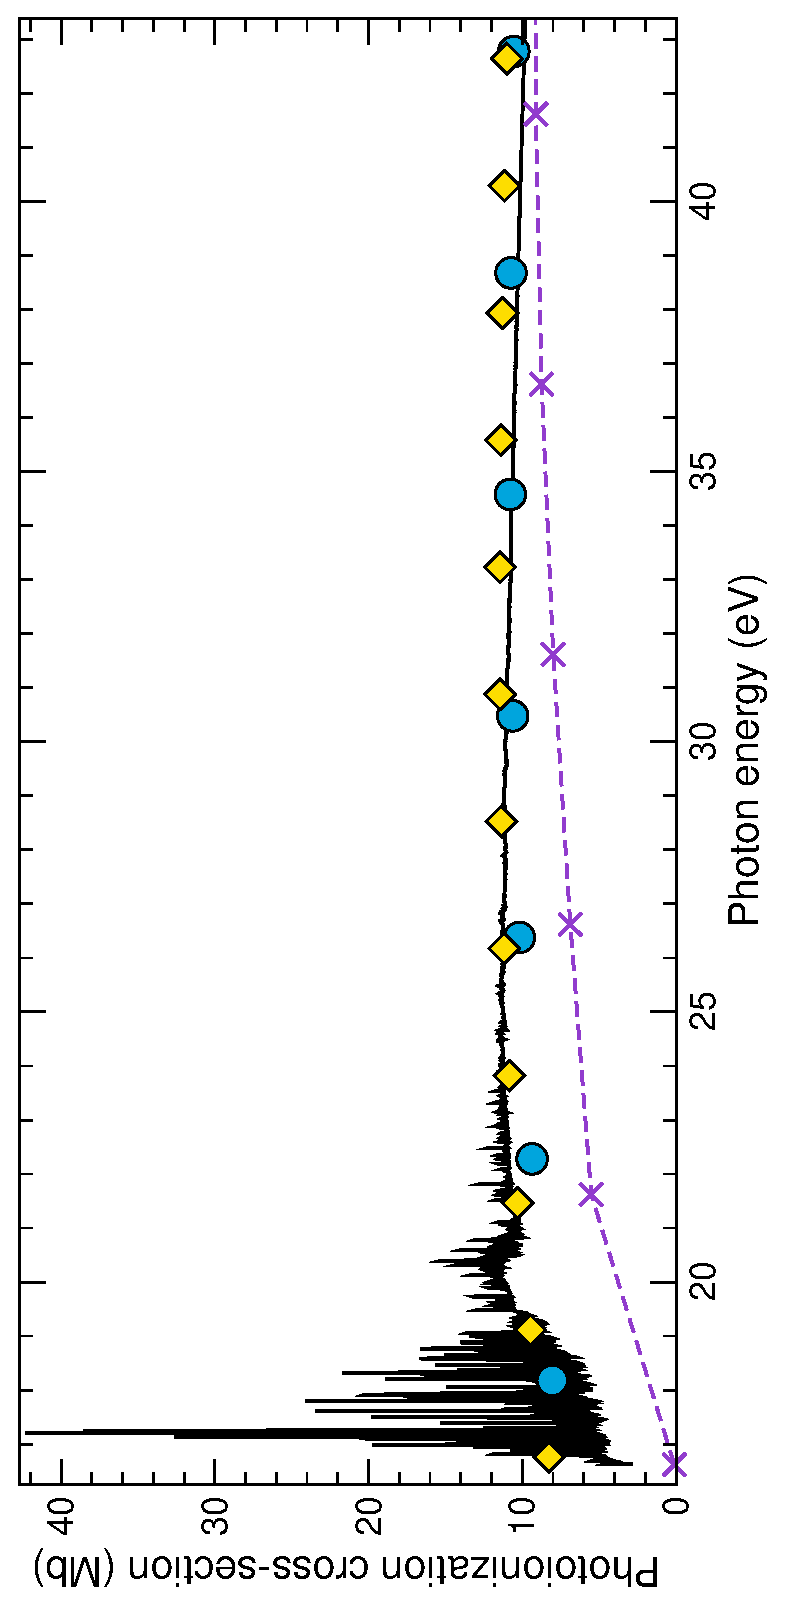
\includegraphics[scale=0.83, angle=-90]{Figures/Cobalt/photo/ground.eps}
\caption{Photoionization cross-sections in Mb against the photon energy in eV. The solid black curve is the total initial ground state, statistically weighted 3d$^8$ $^3$F to all allowed dipole final states. The crosses are results from \citet{1979ApJS...40..815R}, the diamonds are from \citet{1993ADNDT..55..233V}, and finally the circles are those from the distorted wave calculation. \citep{2015JPhB...48n4014F} \label{fig:co_ground}}
\end{sidewaysfigure}
%%%%
%%%
%%
%

%
%%
%%%
%%%%
\begin{sidewaysfigure}
\centering
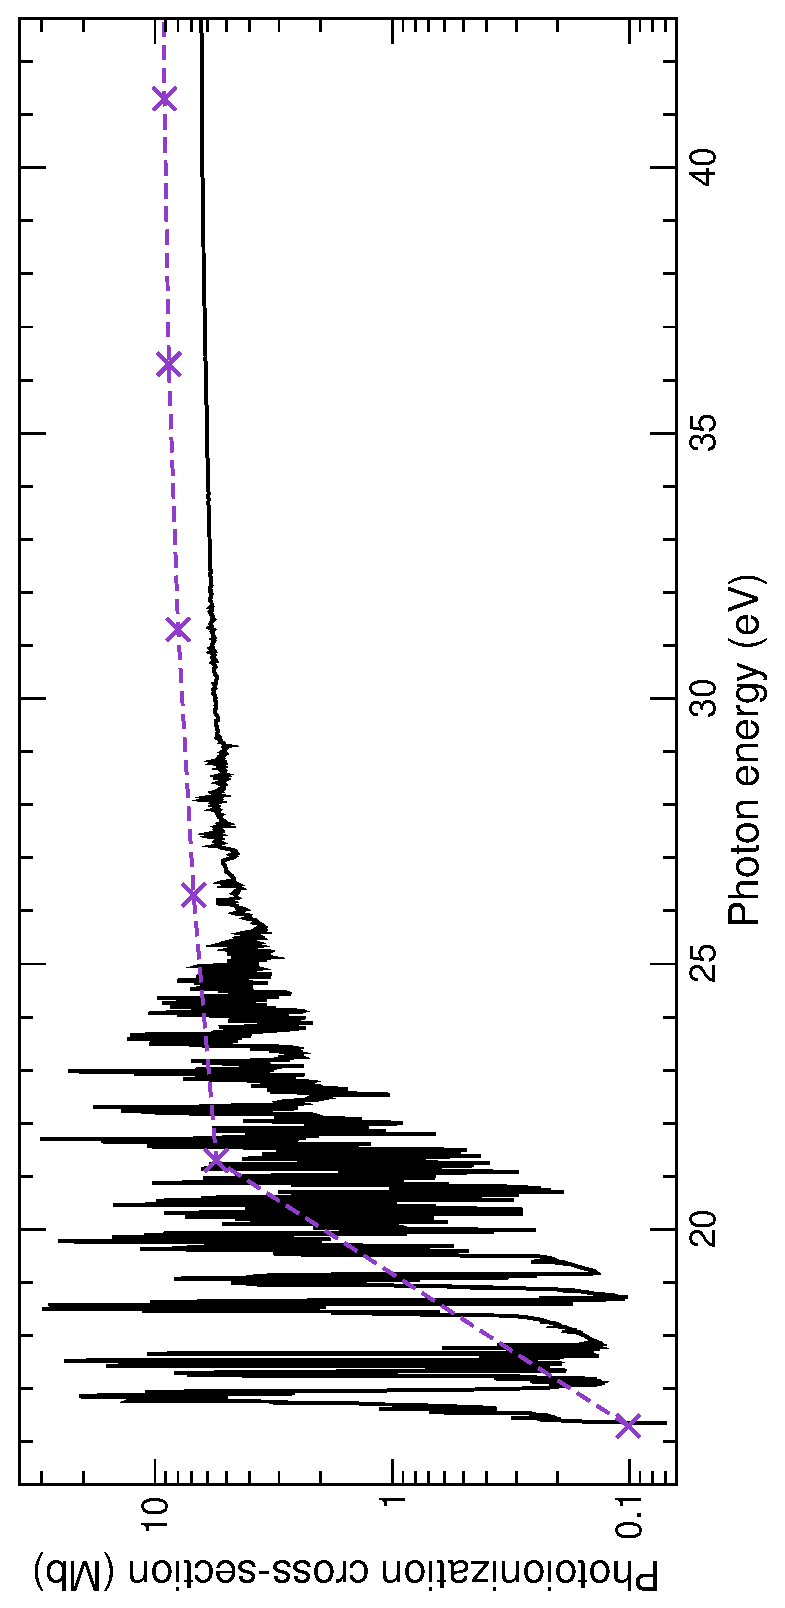
\includegraphics[scale=0.83, angle=-90]{Figures/Cobalt/photo/meta.eps}
\caption{Photoionization cross-sections in Mb against the photon energy in eV. The solid black curve is the photoionization, statistically averaged levels of 3d$^7$4s $^5$F to all allowed dipole final states. The crosses are results from \citet{1979ApJS...40..815R}. \label{fig:co_excited}}
\end{sidewaysfigure}
%%%%
%%%
%%
%

In Figure \ref{fig:co_ground} we present the photoionization cross-section representing the statistically weighted initial state 3d$^8$ a$^3$F to all allowed final states. The results in this figure have been convoluted with a 10 meV Gaussian profile at full-width half-maximum to better compare with experimental results when possible. We directly compare here with the results of all three previously mentioned theoretical methods \citep{1979ApJS...40..815R, 1993ADNDT..55..233V, 2015JPhB...48n4014F}. Previous methods do not include autoionization states and therefore only background cross-sections are presented. It is clear however that the results are in excellent agreement, with only \citet{1979ApJS...40..815R} reaching factors of two or more difference in the $< 20$ eV region. As over 200 eigenenergies obtained from {\sc grasp}0 are $<$ 28 eV of photon energy, this above threshold region is dominated by multiple Rydberg resonances series converging onto these states. 

The second statistically weighted bound state a$^5$F of Co$^{+}$ is from the configuration 3d$^7$4s. In Figure \ref{fig:co_excited} we present the total photoionization cross-section for this metastable level and compare with the earlier work of \citet{1979ApJS...40..815R}. 
This cross-section is weighted as a consequence of its five fine-structure split levels $1 < J < 5$. Again, the photoionization of the $3d$ electron is favourable, so we expect the majority of the spectrum to be accounted for from the 3d$^6$4s target states, which are accessible at 5.75762 eV above the ionization threshold. Good agreement is found between the two calculations for the background cross-section, particularly in the higher photon energy range above 25 eV.

Finally, we often want to determine the partial contribution arising from the recombination process as outlined in Section \ref{sec:spe_rranddr}. We therefore use our photoionization cross-sections and convert them to recombination cross-sections following equation (\ref{eq:spe_milne}) to obtain unified RR+DR rate coefficients defined by equation (\ref{eq:spe_formalrate}). The photoionization from the lowest three initial bound states to the ground 3d$^7$  a$^4$F$_{9/2}$ are provided in Figure \ref{fig:co_rates} a), alongside their respective recombination rates, as a function of electron temperature in Figure \ref{fig:co_rates} b). While we do not carry out any radiative transport calculation involving these rates, it is in our interest to provide such analysis in the future.

%
%%
%%%
%%%%
\begin{sidewaysfigure}
\centering
\begin{subfigure}{0.45\textwidth}
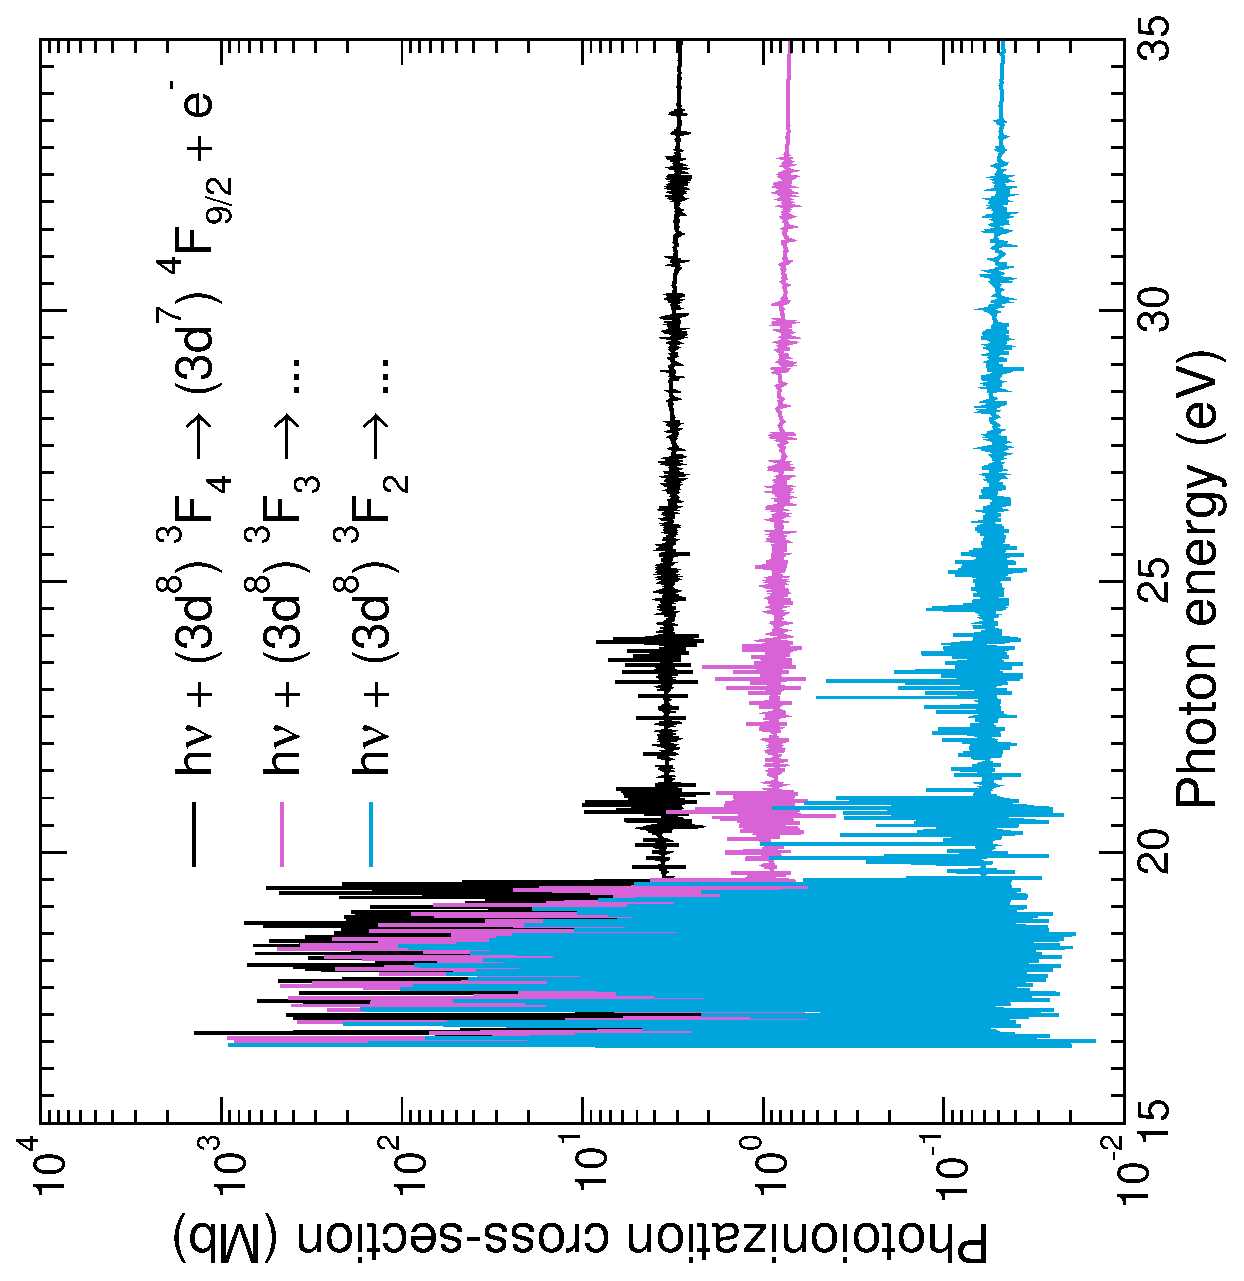
\includegraphics[scale=0.5, angle=-90]{Figures/Cobalt/recomb/recomb_photo.eps}    \end{subfigure}
    ~ %add desired spacing between images, e. g. ~, \quad, \qquad, \hfill etc. 
      %(or a blank line to force the subfigure onto a new line)
    \begin{subfigure}{0.45\textwidth}
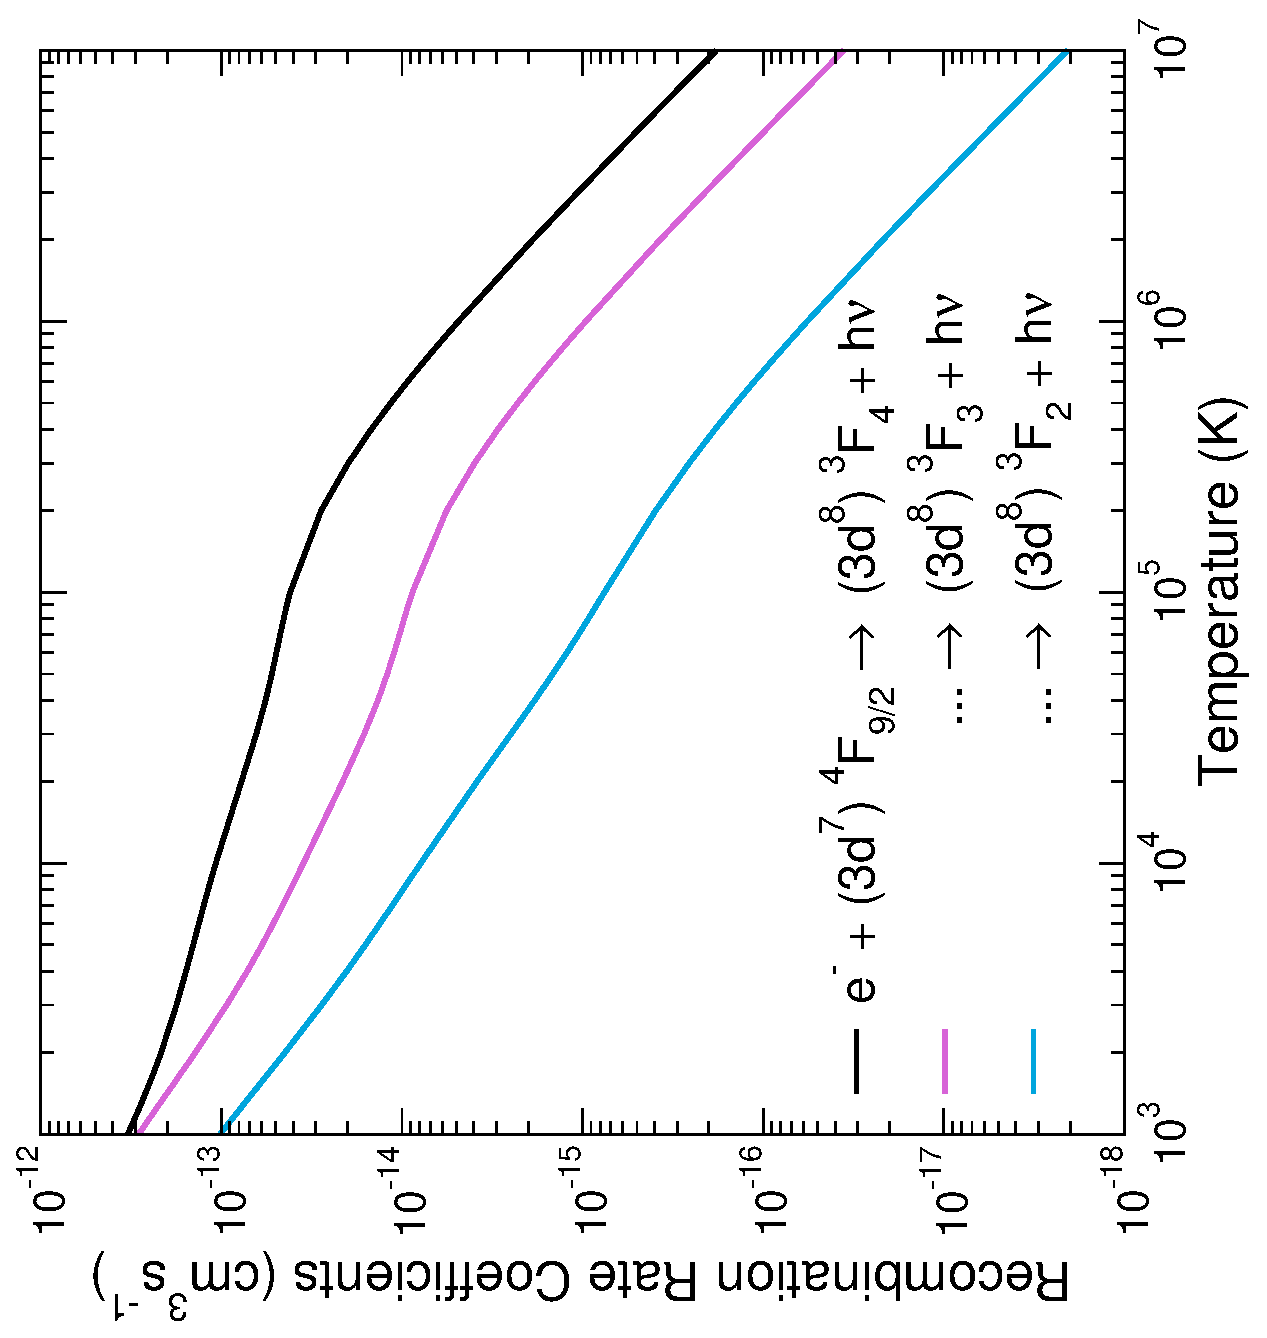
\includegraphics[scale=0.5, angle=-90]{Figures/Cobalt/recomb/total.eps}
    \end{subfigure}
\caption{We present the photoionization cross-section as a function of the photon energy in eV. Three transitions are provided, corresponding to contribution from the lowest three initial bound states into the final ground state 3d$^7$ $^4$F$_{9/2}$. Also presented are the recombination rate coefficients in cm$^3$s$^{-1}$ as a function of electron temperature in K. The transitions are from the initial  3d$^7$ $^4$F$_{9/2}$ state into the three lowest bound states. \label{fig:co_rates}}
\end{sidewaysfigure}
%%%%
%%%
%%
%

\newpage

\subsection{Electron-impact excitation}
The procedures outlined in Section \ref{sec:co_electron} are now applied to obtain accurate collision strengths and the corresponding effective collision strengths describing the electron-impact excitation of Co$^{2+}$. There has been work carried out recently on both singly ionized Co$^{+}$ \citep{2016MNRAS.456.1974S} and also Co$^{2+}$ \citep{2016MNRAS.tmp..556S}. The work of \citet{2016MNRAS.tmp..556S} is similar to our current evaluation, but differences are evident in the method considered. Their basis set has been optimized using {\sc autostructure}, and also includes a $4\bar{d}$ orbital plus additional configuration-interaction. However, only a total of 109 fine-structure levels have been included in the close coupling target representation. The semi-relativistic Breit-Pauli $R$-matrix approach was considered during the scattering calculation.

It is necessary to obtain a level of convergence in the spectra of collision strengths by applying a mesh with incremental step sizes in electron energy until convergence is achieved. Initially 5,000 equally spaced energy points were considered and it was found by the time we had reached 40,000 energy points, the $\Upsilon$'s had converged for these low lying forbidden transitions among the 292 levels. We present in Figure \ref{fig:co_adfcomp} the ratio of these $\Upsilon$'s between a mesh size of 20,000 and 40,000 energy points for level indices lower than 40 and three select temperatures, $T=3,980$ K, $T=10,000$ K, and $T=39,800$ K. The $\%$ difference is $\approx$ 2.7\% between the lowest 40 levels, and $\approx$ 3.34\% between the lowest 100 levels. 

 To extend the energy region we incorporated an additional coarse mesh above the last valence threshold. Due to the long range nature of the Coulomb potential, further contributions to the collision strengths arise from the higher partial waves, particularly for the dipole allowed lines. We compute these additional contributions using the \citet{1992A&A...254..436B} sum rule as well as a geometric series for the long-range non-dipole transitions. Hence, converged total collision strengths were accurately generated for all 42,486 transitions among the 292 fine-structure levels included in the collision calculation. The corresponding effective collision strengths were obtained by averaging these finely resolved collision strengths over a Maxwellian distribution of electron velocities for electron temperatures ranging from 3,800 to 40,000 K.  

%
%%
%%%
%%%%
\begin{figure}[hbt]
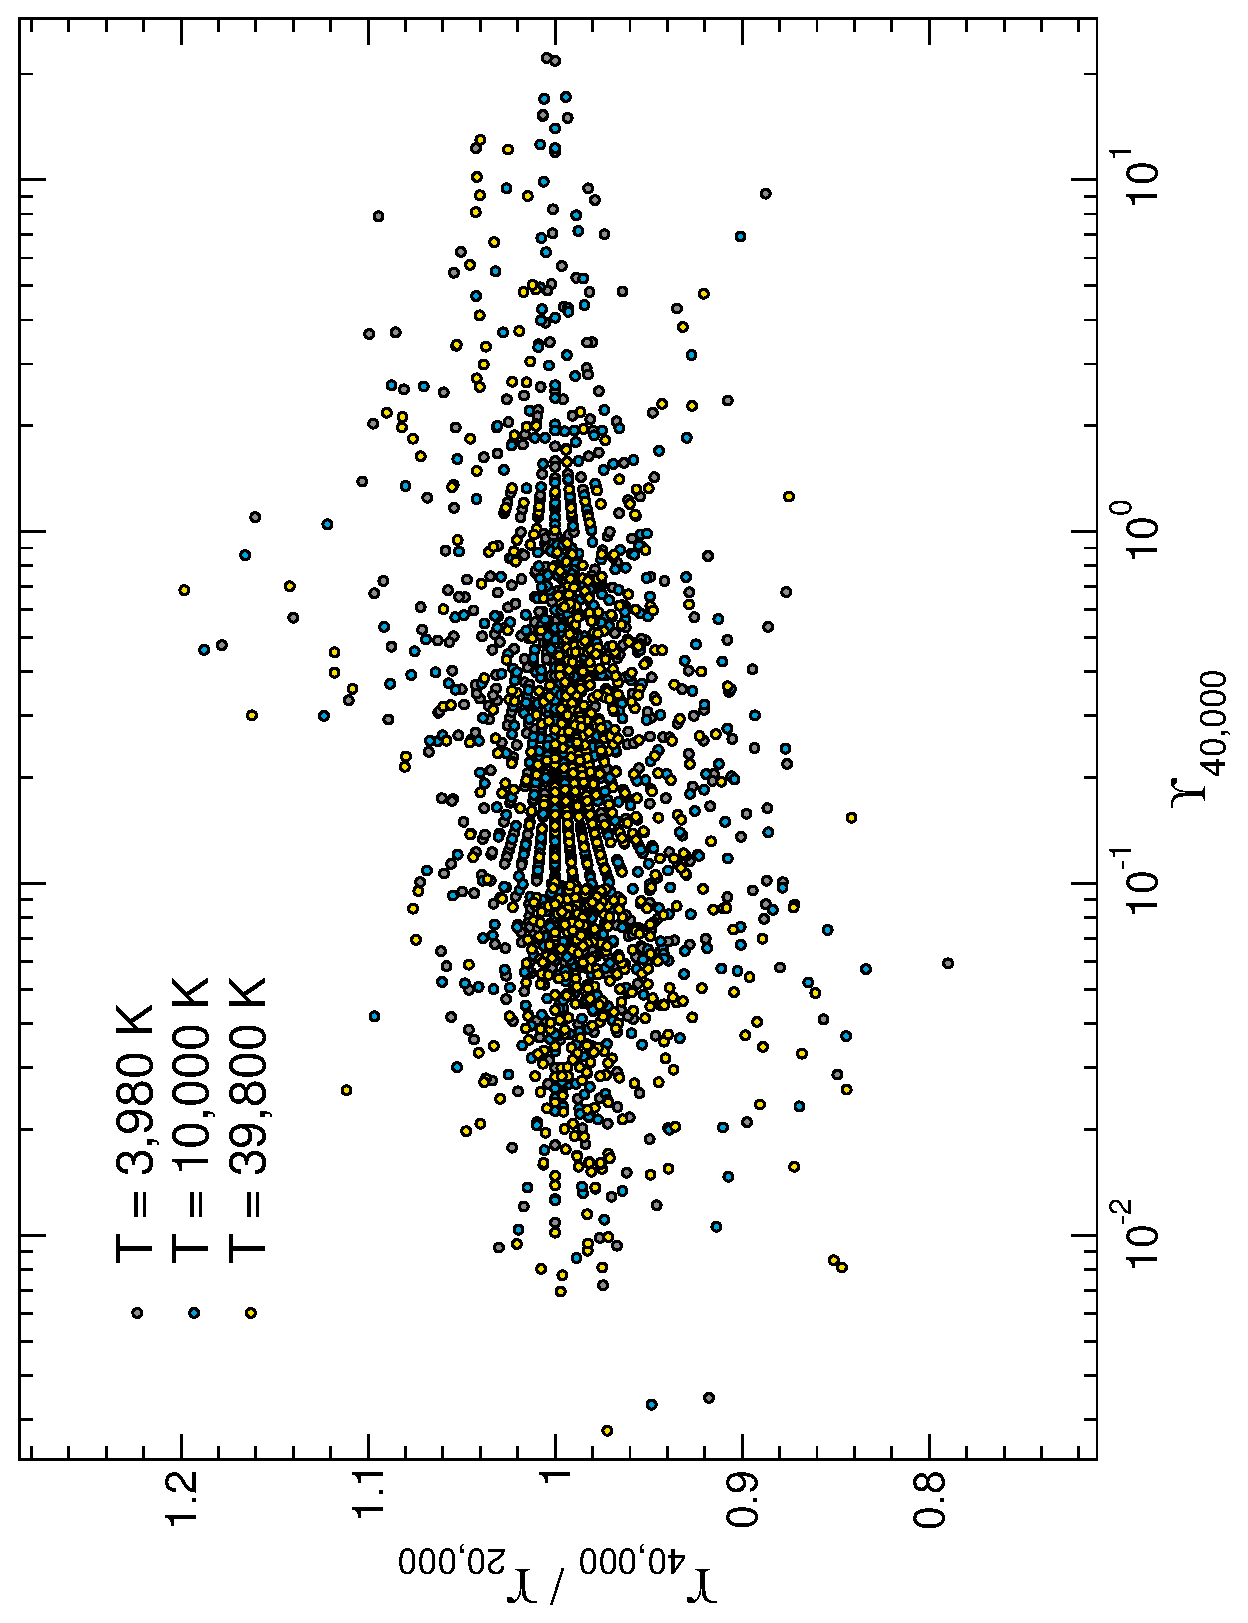
\includegraphics[scale=0.52, angle=-90]{Figures/Cobalt/mesh/adf_compare.eps}
\caption{We present the ratio of effective collision strengths $\Upsilon_{40,000}/\Upsilon_{20,000}$ as a function of the original $\Upsilon_{40,000}$ values. All transitions with level index less than 40 are plotted for three select temperatures of $T=3,980$ K, $T=10,000$ K and $T=39,800$ K. \label{fig:co_adfcomp}}
\end{figure}
%%%%
%%%
%%
%

We present the resulting collision strengths and effective collision strengths for a selection of the forbidden near infrared transitions involving the fine-structure split levels of the $^4$F ground state of Co$^{2+}$. Figure \ref{fig:co_coll_infra1} represents the transition from level 1$\rightarrow$ 2, Figure \ref{fig:co_coll_infra2} is transition $1 \rightarrow 3$, and Figure Figure \ref{fig:co_coll_infra3} is the transition $2 \rightarrow 3$. The collision strength is strongest here for $\Omega_{1 \rightarrow 2}$ due to the $\Delta J = 0$ partial wave. Comparison of the effective collision strengths are made for each transition with the work of \citet{2016MNRAS.tmp..556S} and good agreement is found for all temperatures above 10,000 K. For temperatures below this value the two calculations deviate somewhat, most probably due to the differing resonance profiles converging onto differing threshold positions. The present calculation has shifted the thresholds to lie in their exact observed positions listed in Table \ref{tab:co_energy} whereas the \citet{2016MNRAS.tmp..556S} evaluations do not mention any adjustments.

%
%%
%%%
%%%%
\begin{sidewaysfigure}
\centering
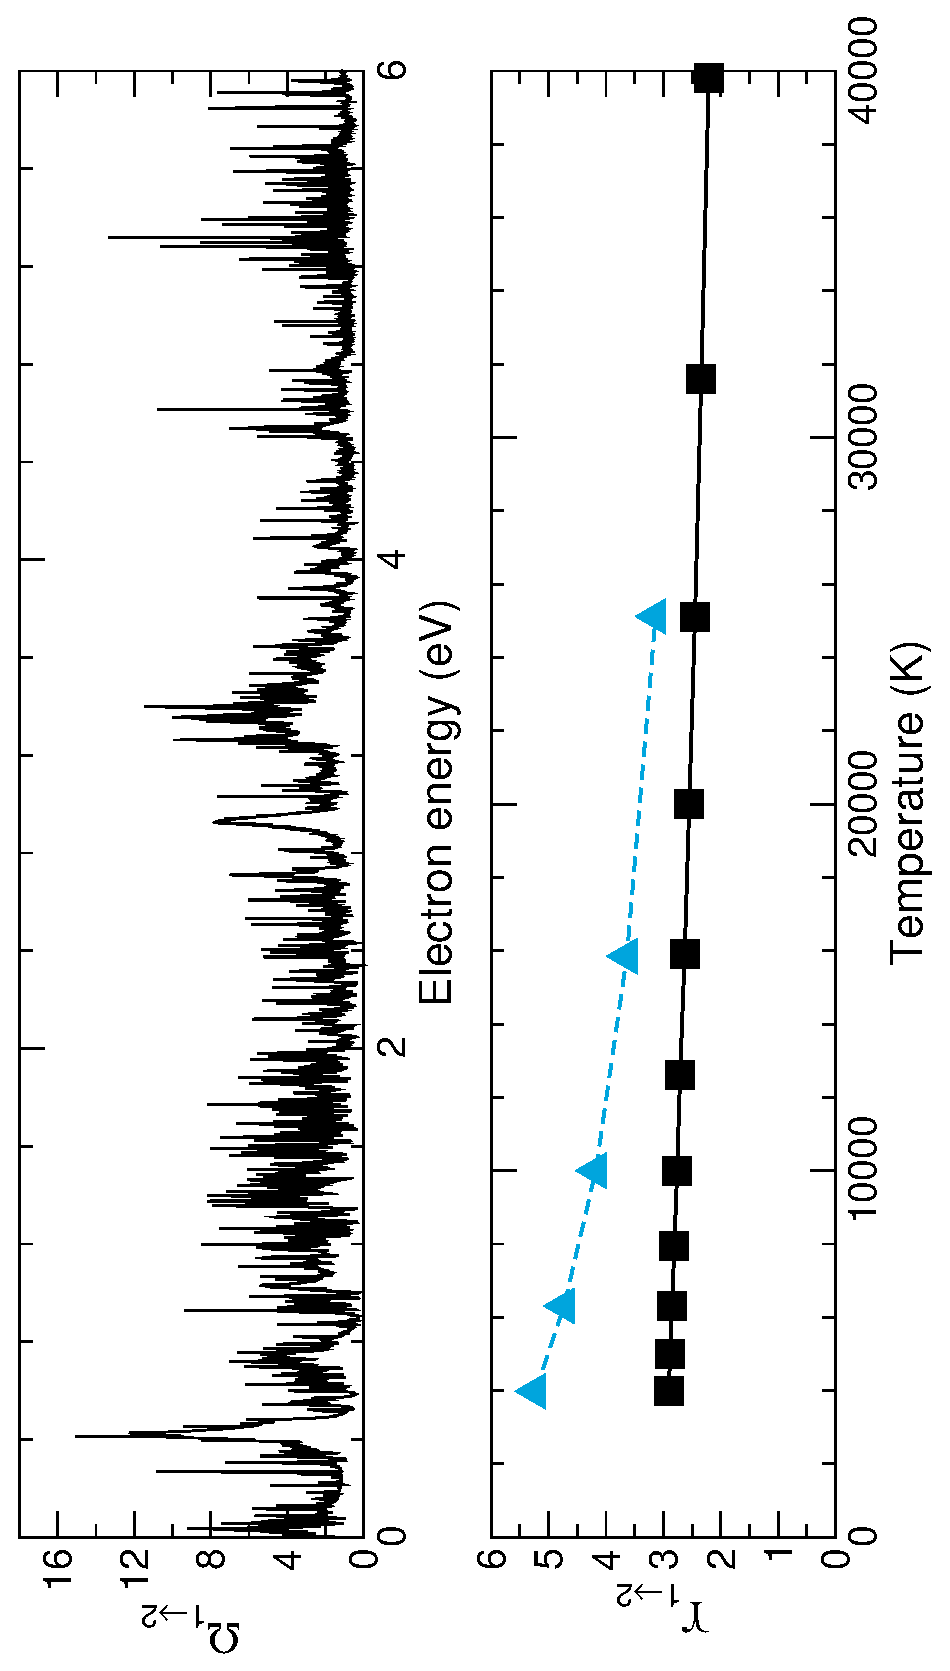
\includegraphics[scale=0.75, angle=-90]{Figures/Cobalt/electron/trans1.eps}
\caption{The collision strength $\Omega_{1\rightarrow 2}$ is presented as a function of electron energy in eV. Also presented are the corresponding effective collision strengths as a function of temperature in K. Solid black lines with squares are the current data set and the dashed blue line with triangles represent the results from \citet{2016MNRAS.tmp..556S}. \label{fig:co_coll_infra1}}
\end{sidewaysfigure}
%%%%
%%%
%%
%

%
%%
%%%
%%%%
\begin{sidewaysfigure}
\centering
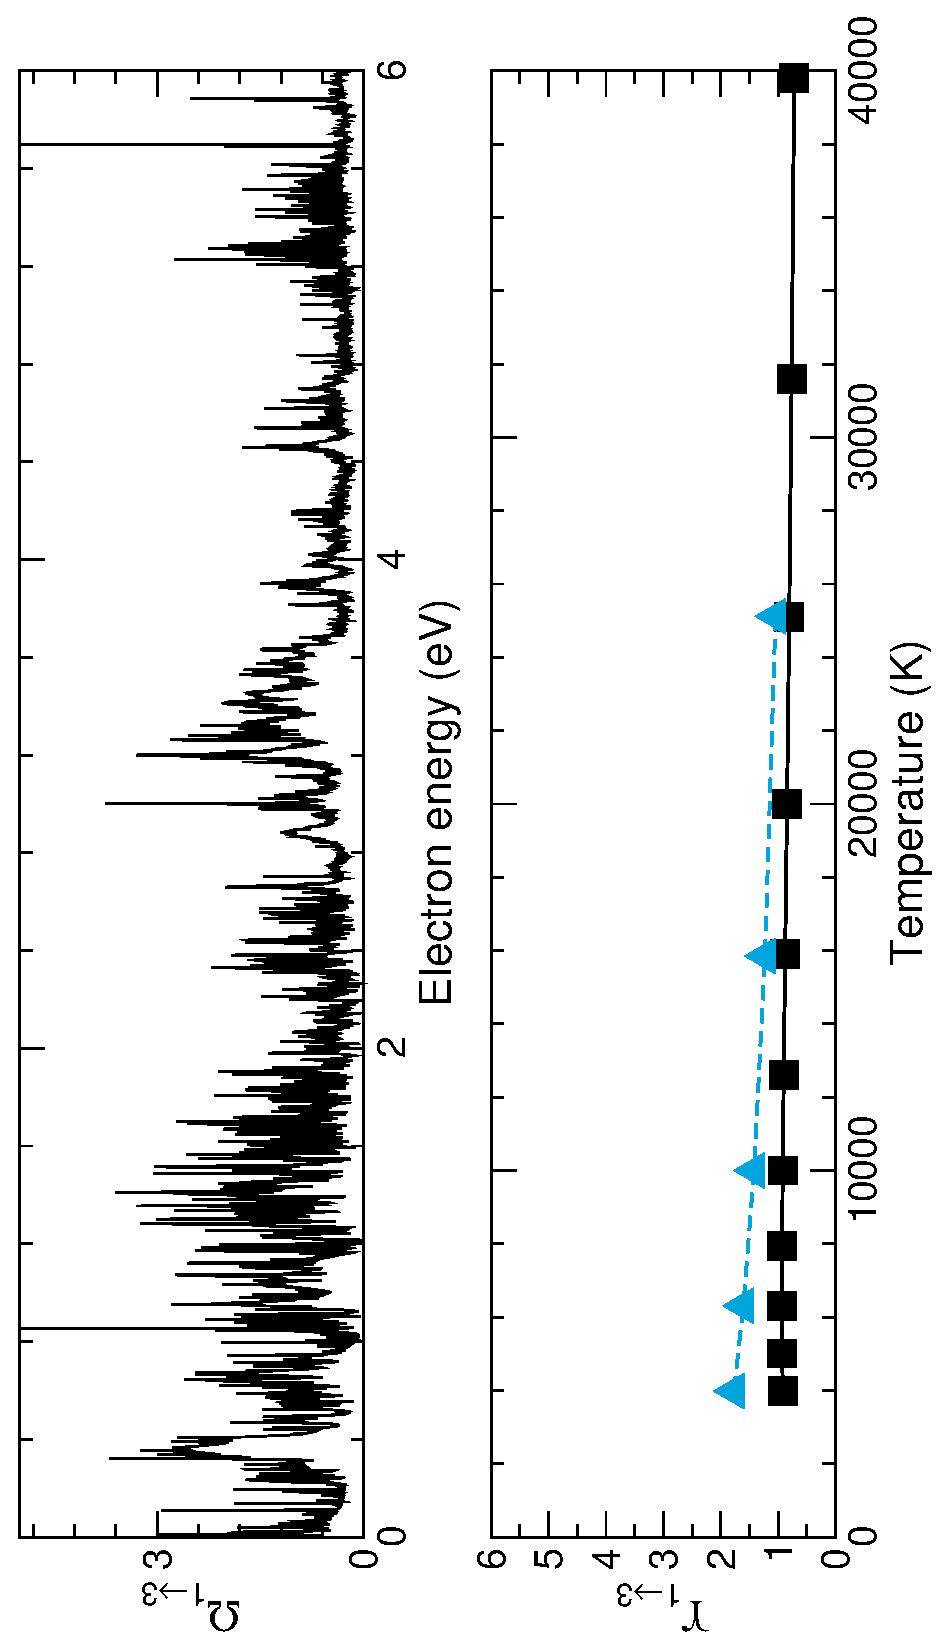
\includegraphics[scale=0.75, angle=-90]{Figures/Cobalt/electron/trans2.eps}
\caption{The collision strength $\Omega_{1\rightarrow 3}$ is presented as a function of electron energy in eV. Also presented are the corresponding effective collision strengths as a function of temperature in K. Solid black lines with squares are the current data set and the dashed blue line with triangles represent the results from \citet{2016MNRAS.tmp..556S}. \label{fig:co_coll_infra2}}
\end{sidewaysfigure}
%%%%
%%%
%%
%

%
%%
%%%
%%%%
\begin{sidewaysfigure}
\centering
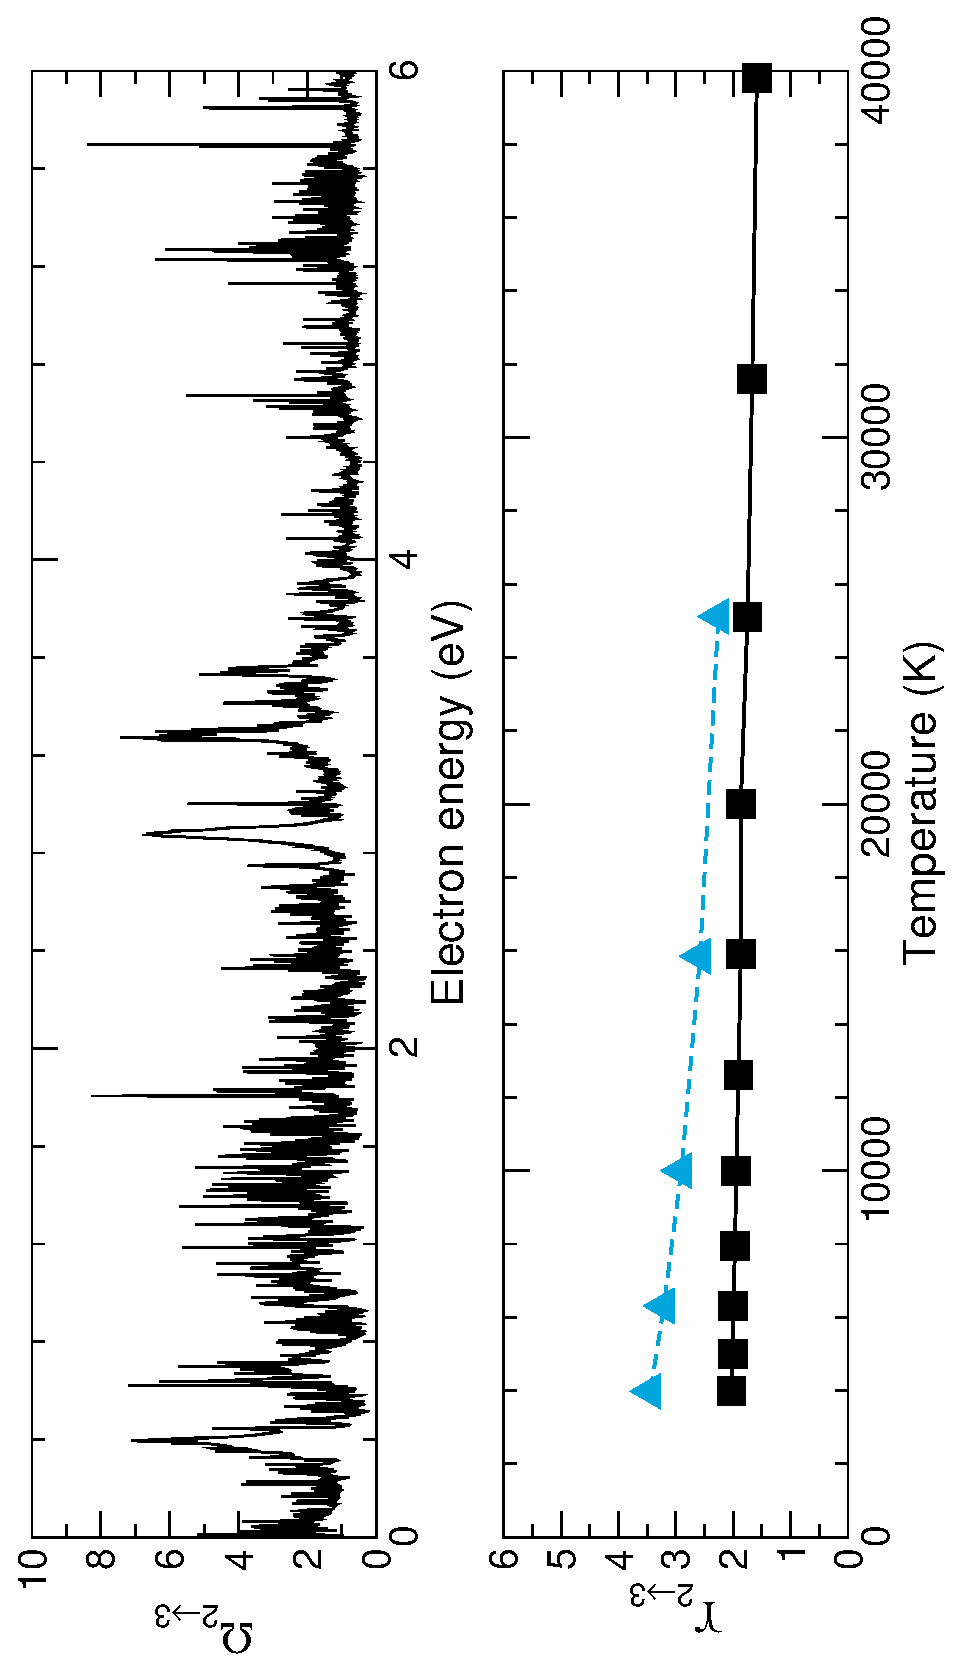
\includegraphics[scale=0.75, angle=-90]{Figures/Cobalt/electron/trans4.eps}
\caption{The collision strength $\Omega_{2\rightarrow 3}$ is presented as a function of electron energy in eV. Also presented are the corresponding effective collision strengths as a function of temperature in K. Solid black lines with squares are the current data set and the dashed blue line with triangles represent the results from \citet{2016MNRAS.tmp..556S}. \label{fig:co_coll_infra3}}
\end{sidewaysfigure}
%%%%
%%%
%%
%

In Figure \ref{fig:co_coll_5to7} we present the effective collision strengths for some higher lying transitions, the 3d$^7$ $^4$F$_{9/2}$ - 3d$^7$ $^2$G$_{9/2}$ (1 $\rightarrow$ 8), 3d$^7$ $^2$P$_{1/2}$ - 3d$^7$ $^2$H$_{9/2}$ (11 $\rightarrow$ 13) and 3d$^7$ $^2$G$_{7/2}$ - 3d$^7$ $^2$H$_{9/2}$ (9 $\rightarrow$ 13). Excellent agreement is evident for all three transitions when a comparison is made with the data of \citet{2016MNRAS.tmp..556S} across all temperatures where a comparison is possible. We present in Table \ref{tab:co_ups} the effective collision strengths for all transitions among the lowest 10 3d$^7$ fine-structure levels across eight temperatures of astrophysical importance.

%
%%
%%%
%%%%
\begin{figure}
\centering
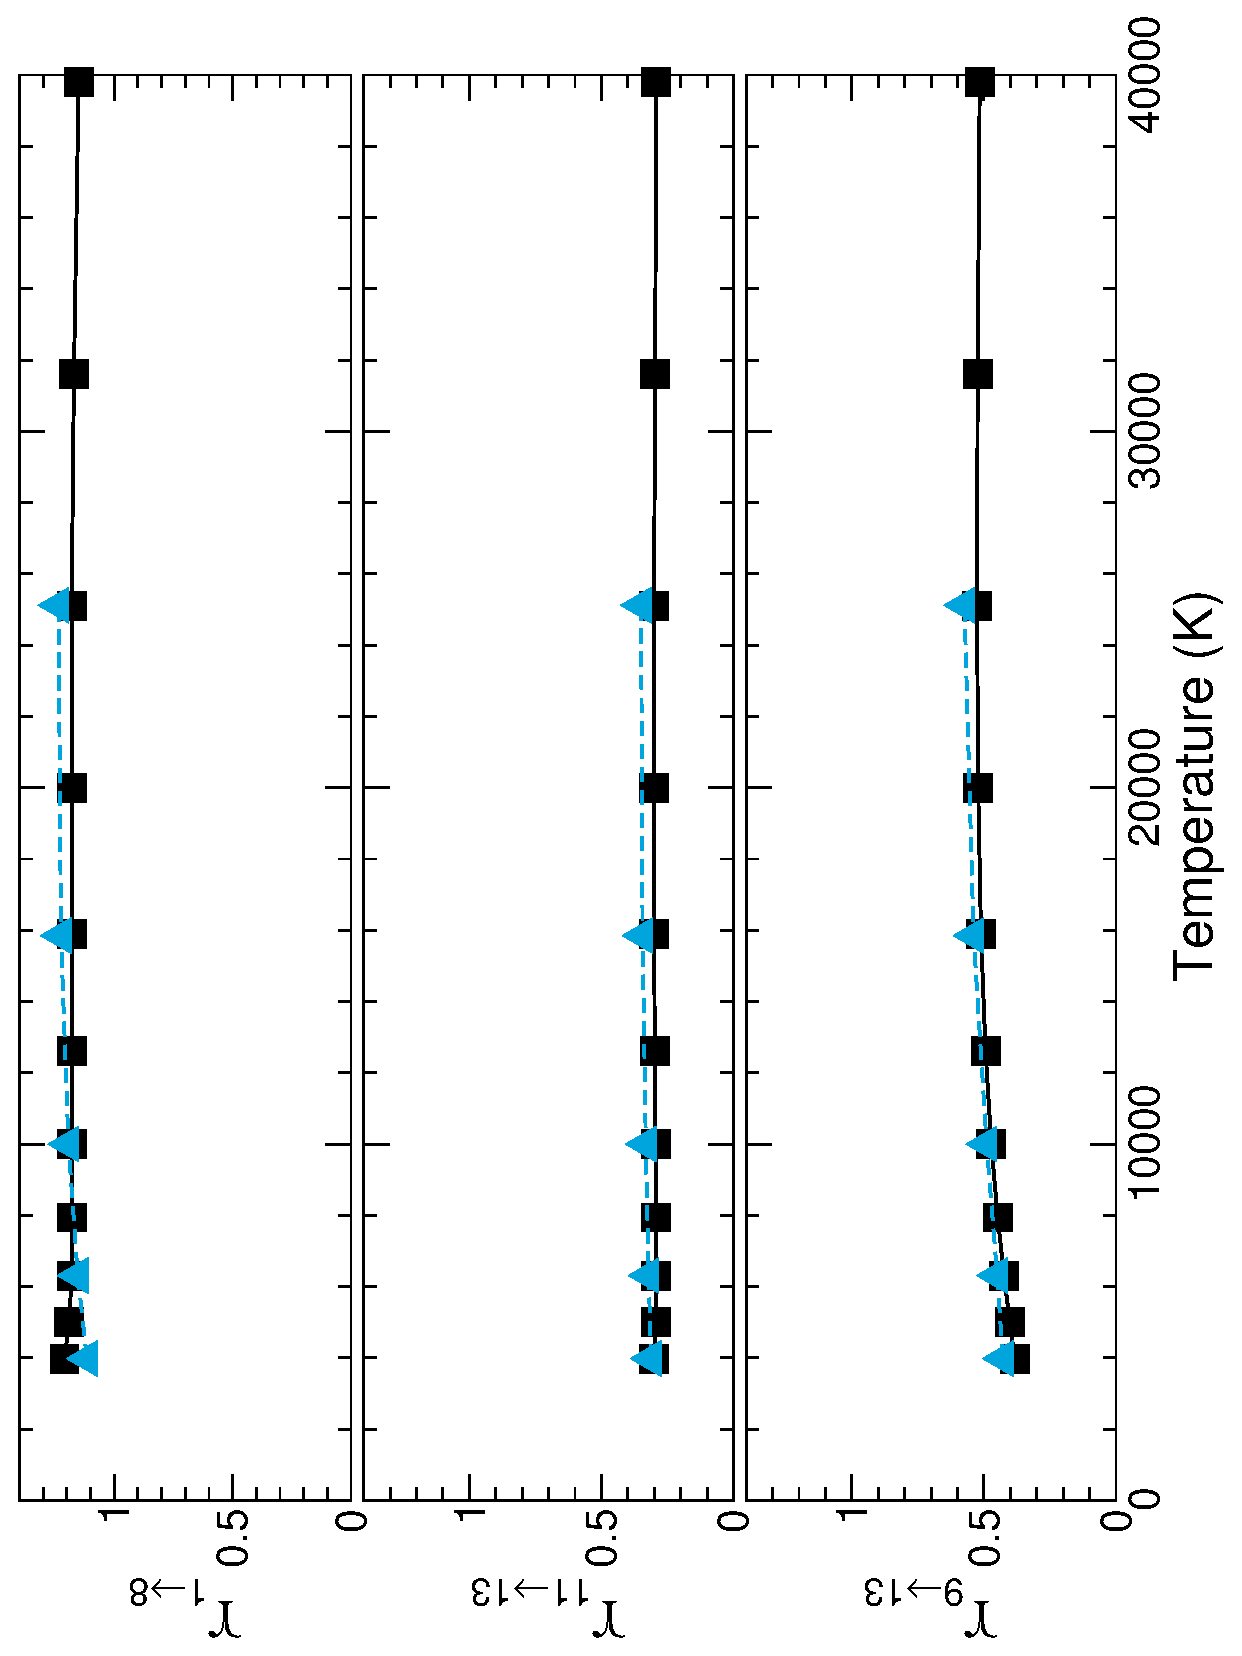
\includegraphics[scale=0.53, angle=-90]{Figures/Cobalt/electron/trans5-7.eps}
\caption{The effective collision strengths, $\Upsilon_{1\rightarrow 8}$ (top), $\Upsilon_{11\rightarrow 13}$ (middle) and $\Upsilon_{9\rightarrow 13}$ (bottom), presented as a function of temperature in K (bottom). Solid black lines with squares are the current data set and the dashed blue line with triangles represent the results from \citep{2016MNRAS.tmp..556S}. \label{fig:co_coll_5to7}}
\end{figure}
%%%%
%%%
%%
%

While we do not compare with the next set of results, we are still able to provide the lowest dipole allowed transitions for completeness, and show the effect from the top-up procedure. In Figure \ref{fig:co_dipole} we present the effective collision strength for the transitions 3d$^6$4p $^6$D$^{{\rm o}}_{9/2} \rightarrow$ 3d$^6$4s $^6$D$_{9/2}$, 3d$^6$4p $^4$D$^{{\rm o}}_{7/2} \rightarrow$ 3d$^7$ $^4$F$_{9/2}$, 3d$^6$4p $^4$D$^{{\rm o}}_{3/2} \rightarrow$ 3d$^7$ $^2$P$_{1/2}$, and 3d$^6$4p $^2$H$^{{\rm o}}_{11/2} \rightarrow$ 3d$^6$4s $^2$H$_{13/2}$ both with (dashed blue), and without (solid black) contribution from top-up. The first transition has a large contribution due to top-up as the quantum numbers are unchanged between initial and final state, $\Delta S = 0$, $\Delta L = 0$, and $\Delta J = 0$. Other transitions have little or no change in their total effective collision strength, but generally any differences occur at temperatures that are beyond the scope of this investigation, i.e. $T>30,000$ K.

\newpage

%
%%
%%%
%%%%
\begin{figure}
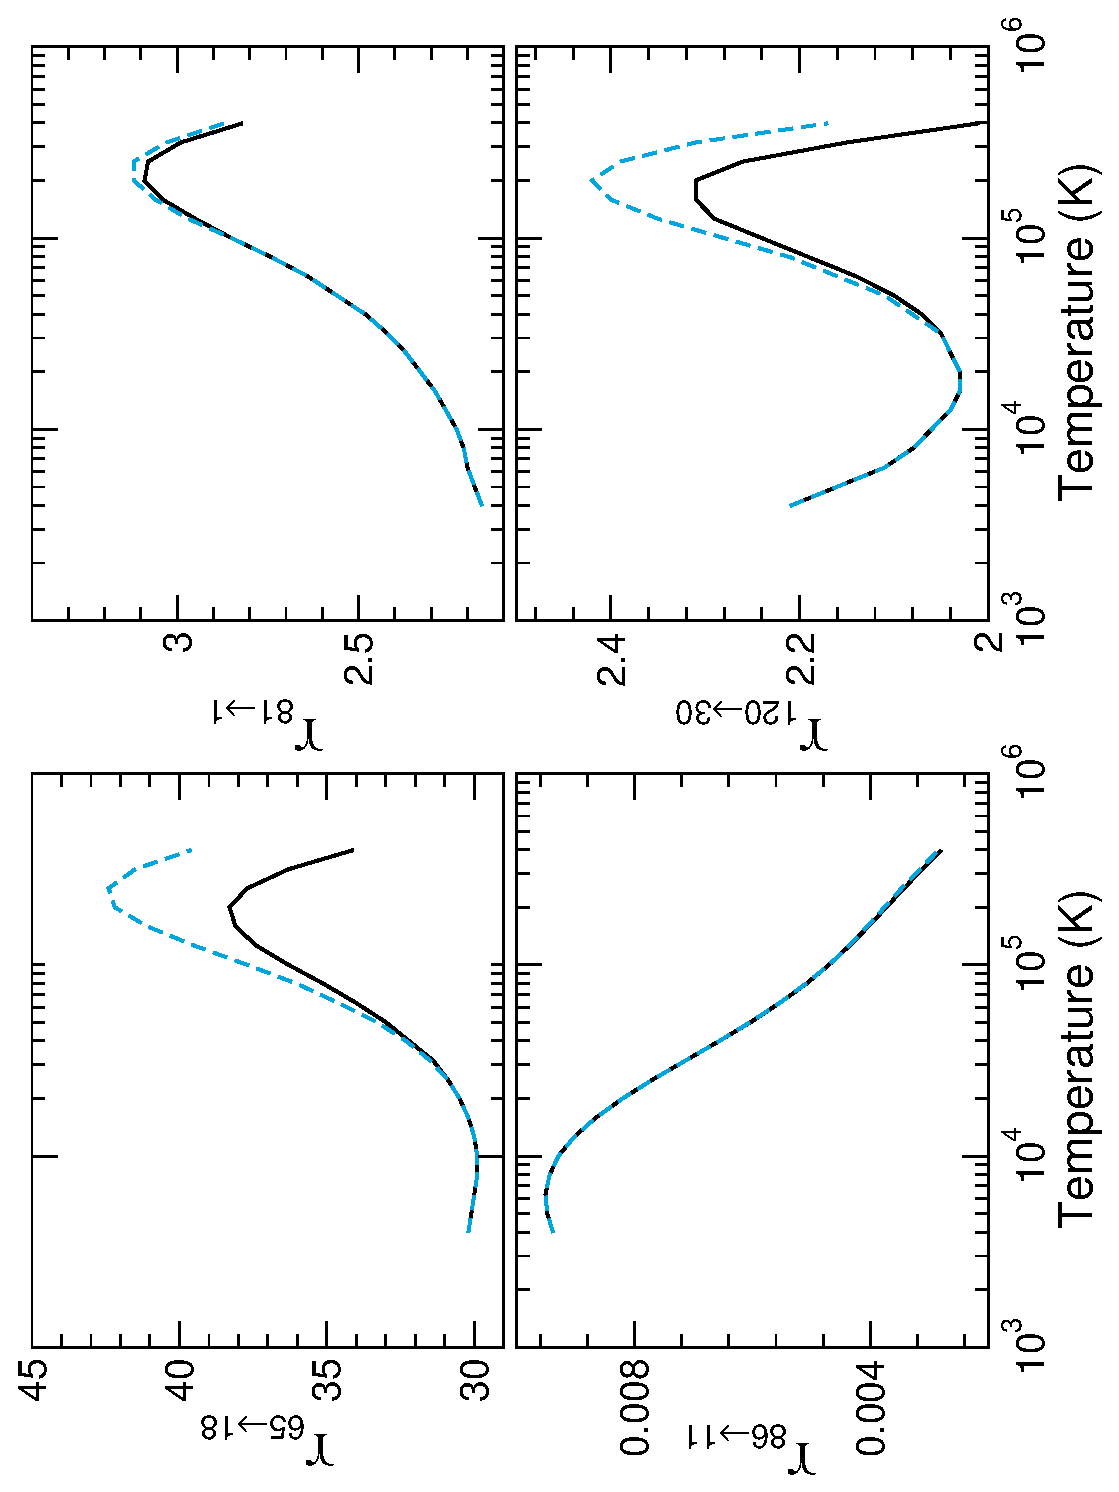
\includegraphics[scale=0.59, angle=-90]{Figures/Cobalt/electron/dipole.eps}
\caption{We present the effective collision strengths according to $\Upsilon_{65\rightarrow 18}$ (top left), $\Upsilon_{81\rightarrow 1}$ (top right), $\Upsilon_{86\rightarrow 11}$ (bottom left), and $\Upsilon_{120\rightarrow 30}$ (bottom right), as a function of electron temperature in K. The solid black curves represent the contribution from the first $J=13$ partial waves (no top-up included) and the dashed blue curves represent the contribution from the remaining partial waves up to $J=38$ (top-up included). \label{fig:co_dipole}}
\end{figure}
%%%%
%%%
%%
%

\subsection{Collisional radiative modelling}\label{sec:co_radiative}
Combining the electron-impact excitation rates with the decay rates ($A$-values), it is possible to study important infrared and visible line ratios from the computer code {\sc collr-v1.0} detailed in Chapter \ref{cha:spectral}. For simplicity and purpose of this study, we neglect the recombination and ionization processes from the neighbouring ion stages and focus on the populating mechanisms solely of Co$^{2+}$.

It is possible to calculate the populations, which are functions of both electron temperature and density, for each of the 262 levels. Due to this quasi-static equilibrium approach $N_1$ is unknown, but since the remaining populations are all relative to $N_1$, we can choose the value to be $1,000$ for example. Populations 2 - 7 are shown in Figure \ref{fig:co_populations} for $T=4,170$, and $T=7,590$, and three densities per temperature; $N_e = 10^4$cm$^{-3}$, $N_e = 10^6$cm$^{-3}$ and $N_e = 10^8$cm$^{-3}$. This reinforces that the problem is not trivial, and the $\Upsilon$'s and $A$-values are of utmost importance.

%
%%
%%%
%%%%
\begin{sidewaysfigure}
\centering
\begin{subfigure}{0.45\textwidth}
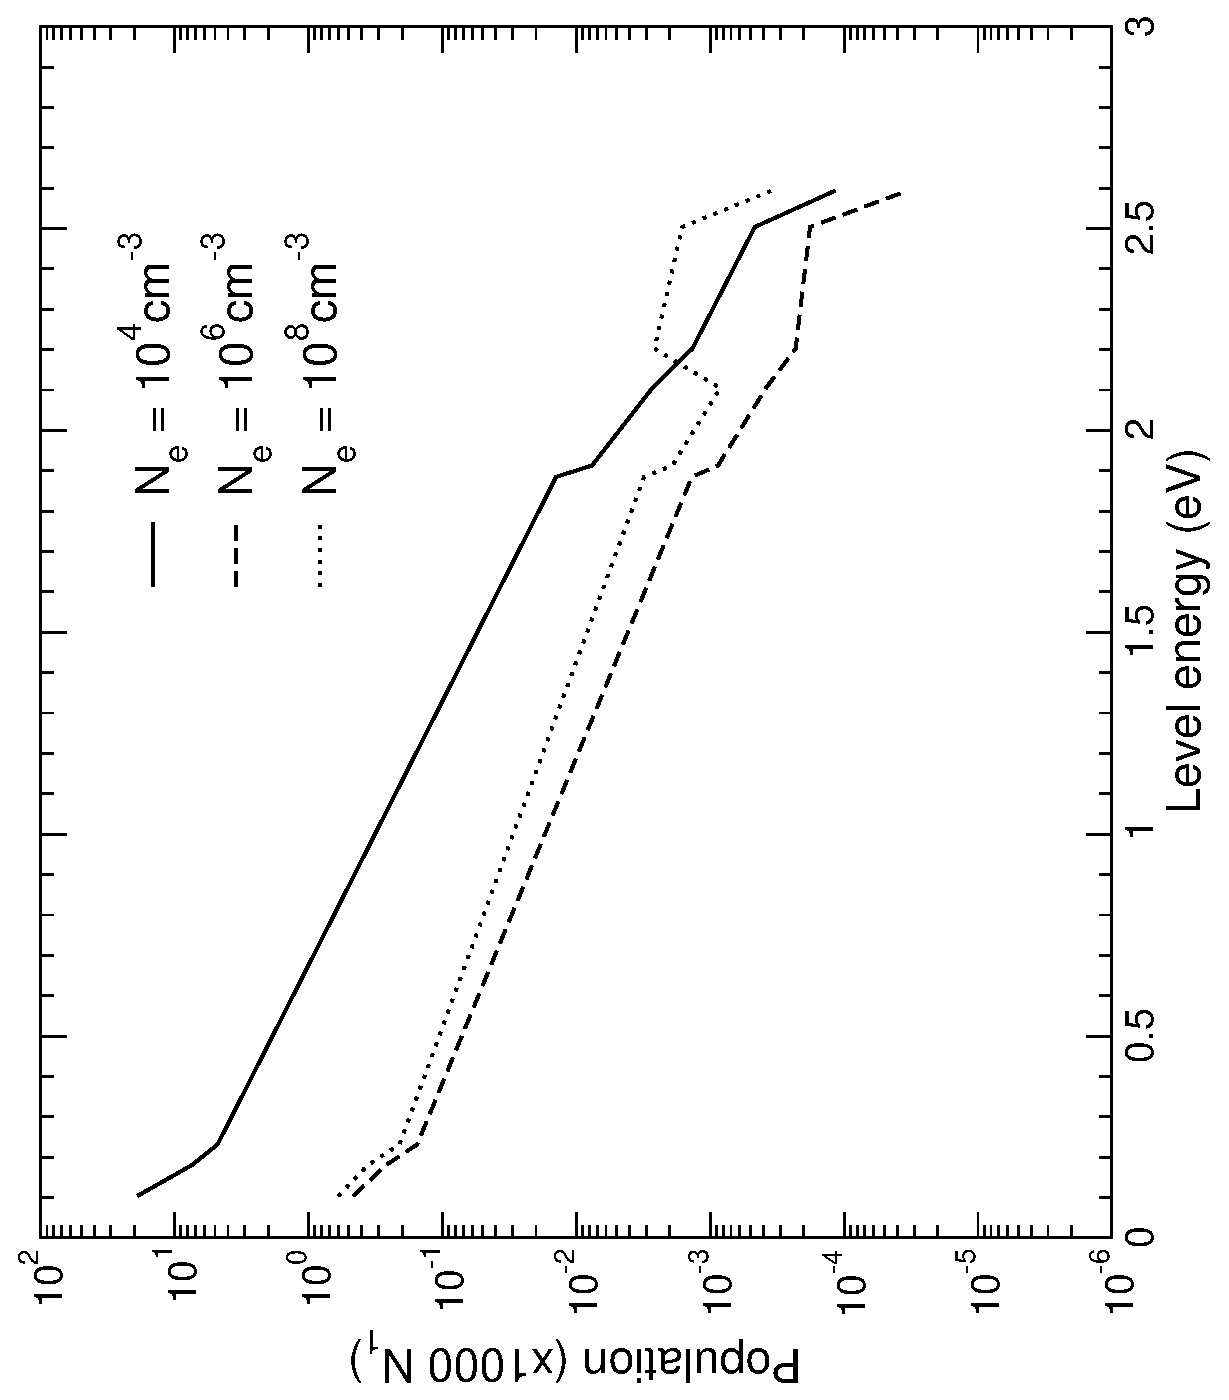
\includegraphics[scale=0.48, angle=-90]{Figures/Cobalt/modelling/populations/population1.eps}    \end{subfigure}
    ~ %add desired spacing between images, e. g. ~, \quad, \qquad, \hfill etc. 
      %(or a blank line to force the subfigure onto a new line)
    \begin{subfigure}{0.45\textwidth}
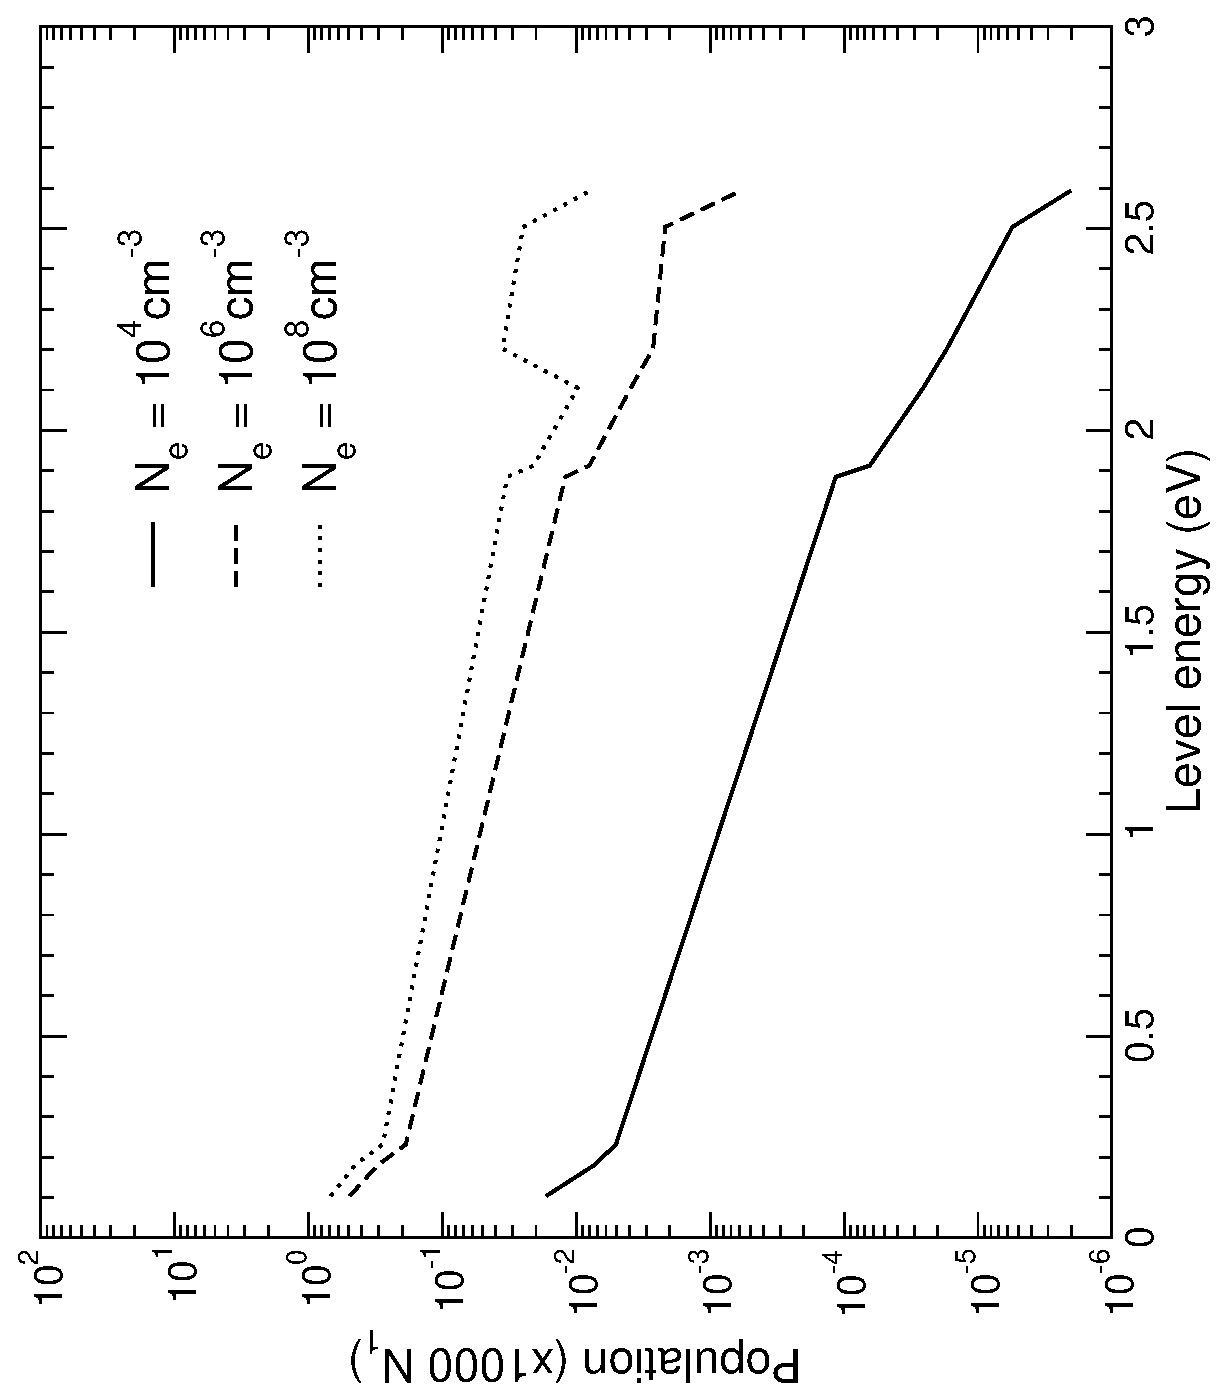
\includegraphics[scale=0.48, angle=-90]{Figures/Cobalt/modelling/populations/population2.eps} 
    \end{subfigure}
\caption{We plot the populations 2 - 7 for $T=4,170$ K (left) and $T=7,590$ K (right) as a function of the target state energies in eV provided by Table \ref{tab:co_energy}, and $N_1 = 1,000$. The populations for each temperature are plotted for three electron densities $N_e = 10^4$cm$^{-3}$, $N_e = 10^6$cm$^{-3}$ and $N_e = 10^8$cm$^{-3}$. \label{fig:co_populations}}
\end{sidewaysfigure}
%%%%
%%%
%%
%

%
%%
%%%
%%%%
\begin{figure}[h]
\centering
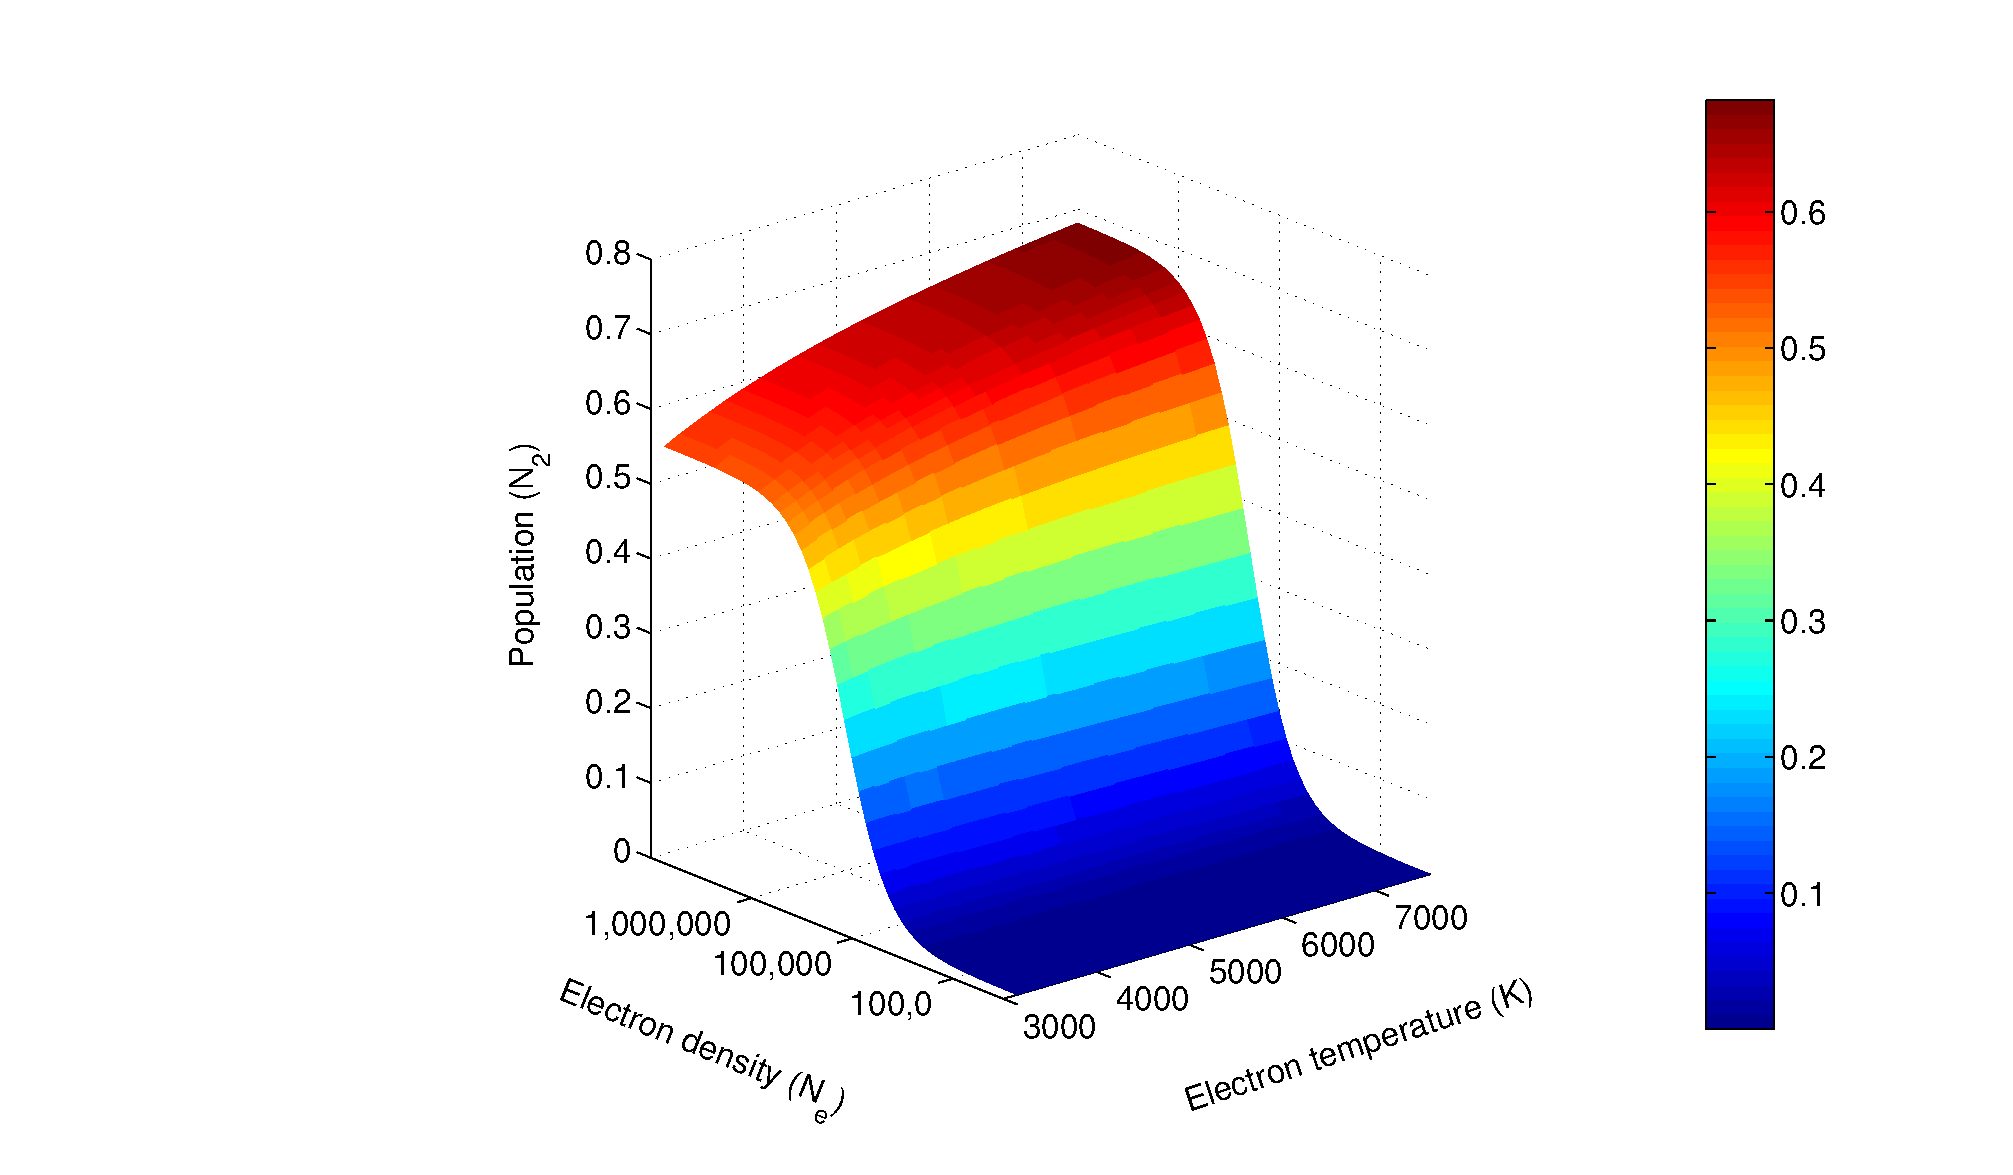
\includegraphics[scale=0.62, angle=0]{Figures/Cobalt/modelling/population2-v2}
\caption{We present the surface plot of $N_2$ in terms of $N_1$ for logarithmic grids of the electron density (cm$^3$) and temperature (K). The resulting population is the corresponding $z$-axis. \label{fig:co_pop2}}
\end{figure}
%%%%
%%%
%%
%
It is also possible to plot particular populations as functions of both electron temperature and density to explain the features in Figure \ref{fig:co_populations}. We therefore present in Figure \ref{fig:co_pop2} the results for a particular population, $N_2$, where we can clearly see the effect of these varying parameters. 

A more useful property to consider is the line ratio as defined in equation (\ref{eq:spe_lratio}). We can therefore investigate select transitions that have been suggested as temperature or density diagnostics. 
%We define the line ratio as
%\[
%\frac{N_j A_{j\rightarrow i}}{N_kA_{k\rightarrow m}},
%\]
%where the populations of the $n^{th}$ level as a function of the ground state are given by $N_n$, and the decay rates are the results from Section \ref{sec:co_target}.

Figure \ref{fig:co_consttemp} depicts the results of the line ratio [0.66$\mu$m]/[0.69$\mu$m] which corresponds to the transitions,
\[
\frac{I_{5\rightarrow1}[0.66\mu m]}{I_{6\rightarrow2}[0.69\mu m]} = \frac{3\text{d}^7 ~\text{a}^4\text{P}_{5/2}\rightarrow 3\text{d}^7 ~\text{a}^4\text{F}_{9/2}}{3\text{d}^7 ~\text{a}^4\text{P}_{3/2} \rightarrow 3\text{d}^7 ~\text{a}^4\text{F}_{7/2}},
\]
as a function of electron density for particular temperatures. The dashed line provides the lowest temperature, $T = 3,980$ K, with increasing $T$ to $T = 5,010$ K, $T = 6,310$ K and $T = 7,940$ K. The line ratio is constant for densities $N_e < 10^{4}$ cm$^{-3}$ and also $N_e > 10^{7}$ cm$^{-3}$ for the temperatures considered. This could be considered a useful diagnostic for densities in the range of $10^{4}$ cm$^{-3}$ $< N_e < 3\times10^{5}$ cm$^{-3}$ where it remains constant for increasing temperatures before it reaches its minimum $\approx 5\times 10^{5}$ cm$^{-3}$. We have also shown the results of the low and high electron density limits from equations (\ref{eq:spe_coronal}) and (\ref{eq:spe_lte}) respectively. The coronal approximation is not as accurate (crosses), but we can see that applying a constant shift in the $y$-axis (stars) that it is useful in determining the actual separation between line ratios. 

%
%%
%%%
%%%%
\begin{figure}[h]
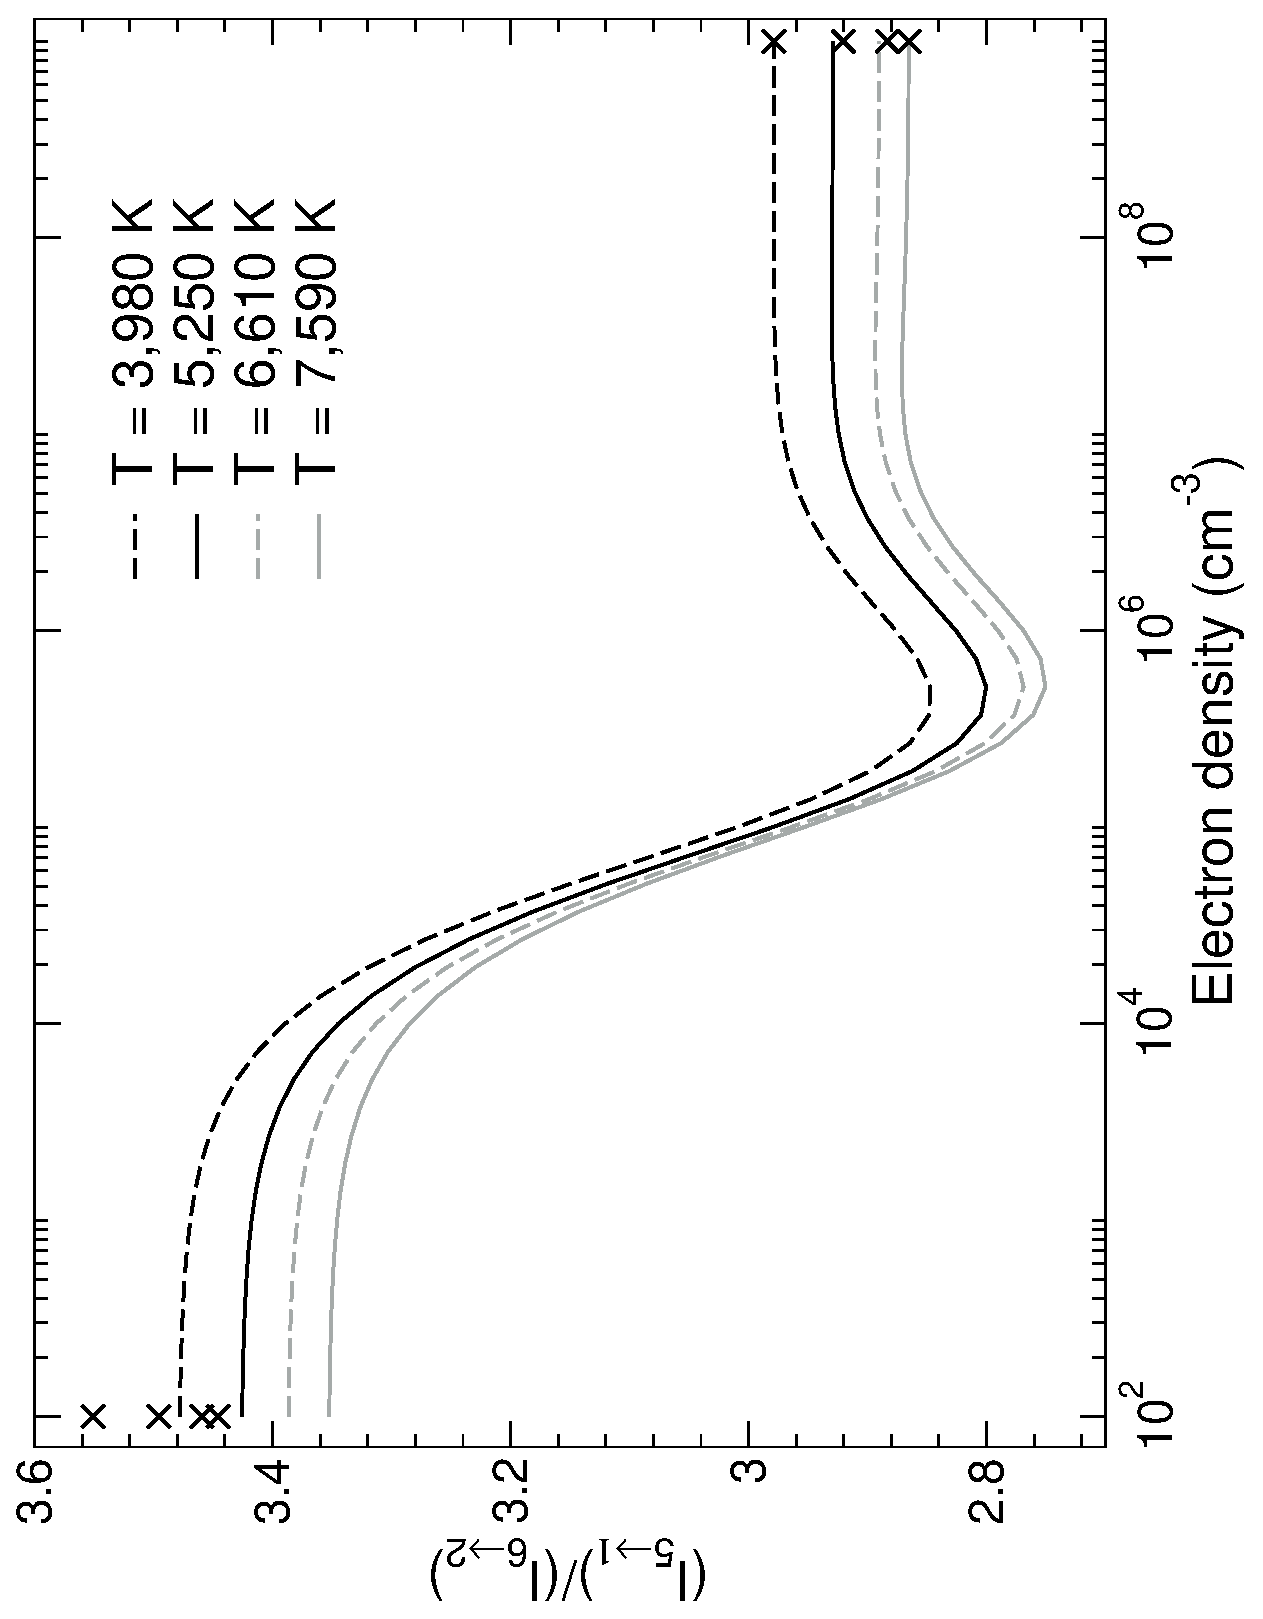
\includegraphics[scale=0.54, angle=-90]{Figures/Cobalt/modelling/5-1over6-2/const_temp.eps}
\caption{The line ratio [0.66$\mu$m]/[0.69$\mu$m] as a function of electron density (cm$^{-3}$). The dashed curve is the lowest temperature, $T = 3,980$ K. The remaining solid black curves are for temperatures $T = 5,010$ K, $T = 6,310$ K, and $T = 7,940$ K for decreasing line ratio. The crosses represent the coronal (low density) and LTE (high density) limits for each of the four temperatures. \label{fig:co_consttemp}}
\end{figure}
%%%%
%%%
%%
%

Next we consider lines suggested by \citet{1995ASPC...78..291R}, (around the wavelength region 6,000 - 6,500 {\rm \AA}) to be applied as density diagnostics. At 10,000 K, we can see the photon emissivity coefficients of the $8\rightarrow 1$ and $8\rightarrow 2$ lines becomes more dominant for increasing temperatures, and they are also in this ideal wavelength region. \citet{2015ApJ...798...93T} also suggests the $2\rightarrow 1$, 11.88$\mu$m as a useful diagnostic line. We finally present the results of three line ratios,
\[
\frac{I_{2\rightarrow 1}[11.88\mu {\rm m}]}{I_{5\rightarrow 1}[0.66\mu {\rm m}]} = \frac{3\rm{d}^7 ~\rm{a}^4\rm{F}_{7/2} \rightarrow 3\rm{d}^7 ~\rm{a}^4\rm{F}_{9/2}}{3\rm{d}^7 ~\rm{a}^4\rm{P}_{5/2} \rightarrow 3\rm{d}^7 ~\rm{a}^4\rm{F}_{9/2}},
\]
\[
\frac{I_{2\rightarrow 1}[11.88\mu {\rm m}]}{I_{8\rightarrow 1}[0.59\mu {\rm m}]} = \frac{3\rm{d}^7 ~\rm{a}^4\rm{F}_{7/2} \rightarrow 3\rm{d}^7 ~\rm{a}^4\rm{F}_{9/2}}{3\rm{d}^7 ~\rm{a}^2\rm{G}_{9/2} \rightarrow 3\rm{d}^7 ~\rm{a}^4\rm{F}_{9/2}},
\]
\[
\frac{I_{2\rightarrow 1}[11.88\mu {\rm m}]}{I_{8\rightarrow 2}[0.62\mu {\rm m}]} = \frac{3\rm{d}^7 ~\rm{a}^4\rm{F}_{7/2} \rightarrow 3\rm{d}^7 ~\rm{a}^4\rm{F}_{9/2}}{3\rm{d}^7 ~\rm{a}^2\rm{G}_{9/2} \rightarrow 3\rm{d}^7 ~\rm{a}^4\rm{F}_{7/2}},
\]


%
%%
%%%
%%%%
\begin{sidewaysfigure}
\centering
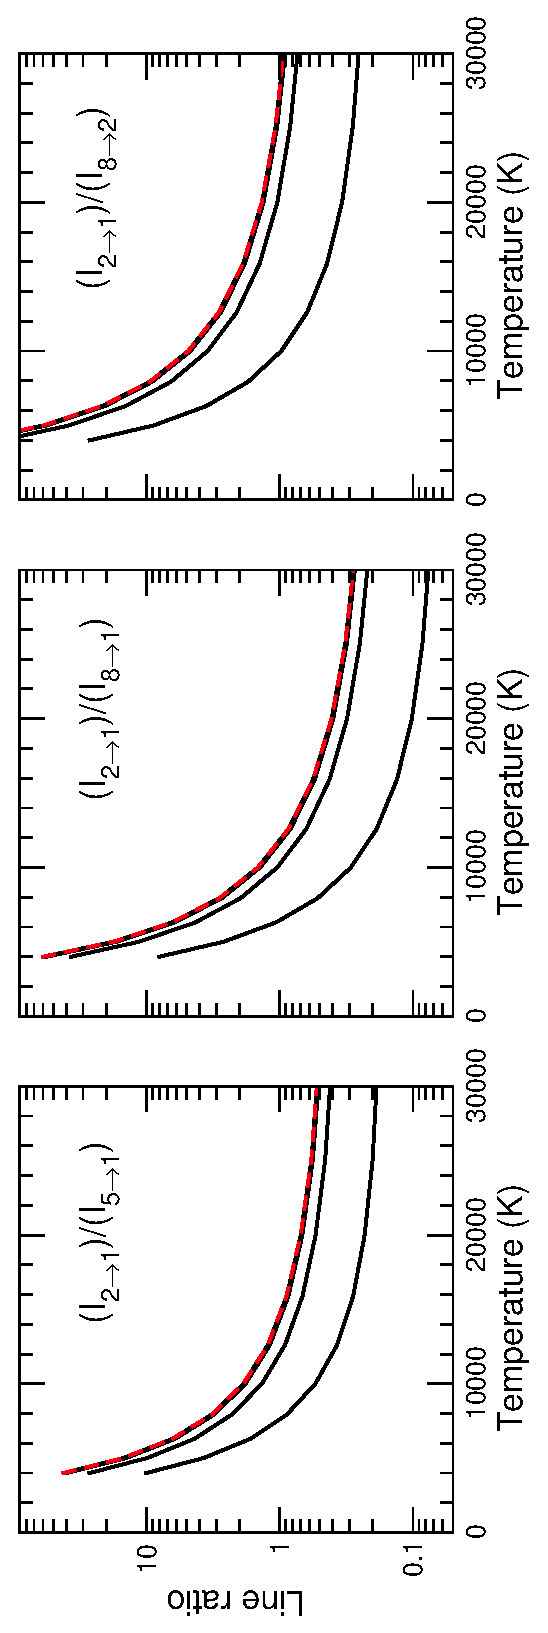
\includegraphics[scale=0.8, angle=-90]{Figures/Cobalt/modelling/lineratio_new.eps}
\caption{Three line ratios of [11.88$\mu$m]/[0.66$\mu$m] (left), [11.88$\mu$m]/[0.59$\mu$m] (middle), and [11.88$\mu$m]/[0.62$\mu$m] (right) as a function of electron temperature (K). The red, dashed curve is the lowest density, $N_e = 10^2$ cm$^{-3}$. The remaining solid black curves are for temperatures $N_e = 10^3$ cm$^{-3}$, $N_e = 10^4$ cm$^{-3}$, $N_e = 10^5$ cm$^{-3}$, and $N_e = 10^6$ cm$^{-3}$ for decreasing line ratio.\label{fig:co_constdens}}
\end{sidewaysfigure}
%%%%
%%%
%%
%


We plot in Figure \ref{fig:co_constdens} the three line ratios as a function of electron temperature. The red dashed curves are the lowest electron density in each Figure - $N_e = 10^2$ cm$^{-3}$, and the remaining solid curves correspond to $N_e = 10^3$ cm$^{-3}$, $N_e = 10^4$ cm$^{-3}$, $N_e = 10^5$ cm$^{-3}$, and $N_e = 10^6$ cm$^{-3}$. Each line ratio is a varying function of increasing temperature across the range of interest. The three lowest densities lie right on top of each other in each plot, and therefore they provide useful diagnostics for this density range. As $N_e > 10^5$ cm$^{-3}$, the line ratio begins to diverge, and even becomes constant for larger densities.

\newpage
\section{Conclusion}\label{sec:co_conclusions}
In this Chapter we present an extensive set of atomic data for the photoionization of Co$^{+}$ and the electron-impact excitation of Co$^{2+}$. Initially we have exploited the computer code {\sc grasp}0 to obtain a description of the atomic wavefunctions and generate energy levels for the 292 fine-structure bound target states and the corresponding $A$-values for transitions between these levels. We compare these levels with the theoretical work of \citet{2016MNRAS.tmp..556S} and the observational study of \citet{1985aeli.book.....S}, which are the values recorded in the NIST database. Furthermore, the {\sc darc} computer package has been employed to extend the problem to include photon and electron interactions. 

We then present statistically weighted, level-resolved ground and metastable photoionization cross-sections for the Co$^{+}$ ion as well as collision strengths and Maxwe-\\llian averaged effective collision strengths describing the electron-impact excitation of the Co$^{2+}$ ion. Comparisons are made with other works where possible and good agreement is found. The reliability of the atomic data presented has been rigorously tested through a variety of means, such as the sophistication of the current calculations where great care has been taken to ensure the inclusion of important correlation and configuration-interaction in the wavefunction expansions. In addition the complex resonance structures in the cross-sections (photoionization and excitation) have been accurately resolved through a series of calculations incorporating mesh sizes with finer and finer energy increments. A proper consideration was also taken of the contributions from the high partial waves to ensure convergence of the collision strengths for the allowed transitions in particular. A conclusive assessment of the accuracy of the presented Maxwellian averaged collision strengths will necessarily come from any subsequent astrophysical or diagnostic application. 

In Section \ref{sec:co_radiative} the electron-impact excitation rates were combined with the decay rates ($A$-values) to investigate important infrared and visible line ratios. During this process we were able to identify useful transitions that could be used as temperature and/or density sensitive diagnostic lines.

\newpage
\begin{table*}
\centering
\footnotesize
\begin{tabular}{c c c c c c c c c c}
\toprule
\multicolumn{2}{c}{ } & \multicolumn{8}{c}{log $T$ (K)} \\
$i$ & $j$   & 3.6 & 3.7 & 3.8 & 3.9 &  4 & 4.1 & 4.2 & 4.3 \\%& 4.4 \\
\midrule
   1 &    2 & $ 2.92^{+00}$ & $ 2.90^{+00}$ & $ 2.86^{+00}$ & $ 2.82^{+00}$ & $ 2.77^{+00}$ & $ 2.70^{+00}$ & $ 2.63^{+00}$ & $ 2.54^{+00}$ \\%& $ 2.44^{+00}$\\
   1 &    3 & $ 9.24^{-01}$ & $ 9.36^{-01}$ & $ 9.41^{-01}$ & $ 9.37^{-01}$ & $ 9.26^{-01}$ & $ 9.06^{-01}$ & $ 8.79^{-01}$ & $ 8.45^{-01}$ \\%& $ 8.06^{-01}$\\
   2 &    3 & $ 2.02^{+00}$ & $ 2.01^{+00}$ & $ 1.99^{+00}$ & $ 1.97^{+00}$ & $ 1.94^{+00}$ & $ 1.91^{+00}$ & $ 1.86^{+00}$ & $ 1.81^{+00}$ \\%& $ 1.74^{+00}$\\ 
   1 &    4 & $ 3.17^{-01}$ & $ 3.23^{-01}$ & $ 3.26^{-01}$ & $ 3.25^{-01}$ & $ 3.21^{-01}$ & $ 3.13^{-01}$ & $ 3.03^{-01}$ & $ 2.90^{-01}$ \\%& $ 2.75^{-01}$\\
   2 &    4 & $ 7.46^{-01}$ & $ 7.65^{-01}$ & $ 7.77^{-01}$ & $ 7.80^{-01}$ & $ 7.76^{-01}$ & $ 7.64^{-01}$ & $ 7.43^{-01}$ & $ 7.17^{-01}$ \\%& $ 6.85^{-01}$\\
   3 &    4 & $ 1.42^{+00}$ & $ 1.42^{+00}$ & $ 1.42^{+00}$ & $ 1.42^{+00}$ & $ 1.40^{+00}$ & $ 1.39^{+00}$ & $ 1.36^{+00}$ & $ 1.32^{+00}$ \\%& $ 1.28^{+00}$\\
   1 &    5 & $ 1.16^{+00}$ & $ 1.16^{+00}$ & $ 1.17^{+00}$ & $ 1.19^{+00}$ & $ 1.20^{+00}$ & $ 1.21^{+00}$ & $ 1.21^{+00}$ & $ 1.20^{+00}$ \\%& $ 1.19^{+00}$\\
   2 &    5 & $ 8.11^{-01}$ & $ 8.03^{-01}$ & $ 8.02^{-01}$ & $ 8.07^{-01}$ & $ 8.13^{-01}$ & $ 8.17^{-01}$ & $ 8.15^{-01}$ & $ 8.05^{-01}$ \\%& $ 7.89^{-01}$\\
   3 &    5 & $ 5.72^{-01}$ & $ 5.60^{-01}$ & $ 5.53^{-01}$ & $ 5.51^{-01}$ & $ 5.50^{-01}$ & $ 5.48^{-01}$ & $ 5.43^{-01}$ & $ 5.33^{-01}$ \\%& $ 5.19^{-01}$\\   
   4 &    5 & $ 3.68^{-01}$ & $ 3.51^{-01}$ & $ 3.37^{-01}$ & $ 3.27^{-01}$ & $ 3.20^{-01}$ & $ 3.13^{-01}$ & $ 3.06^{-01}$ & $ 2.98^{-01}$ \\%& $ 2.88^{-01}$\\    
   1 &    6 & $ 4.84^{-01}$ & $ 4.82^{-01}$ & $ 4.84^{-01}$ & $ 4.90^{-01}$ & $ 4.95^{-01}$ & $ 4.98^{-01}$ & $ 4.97^{-01}$ & $ 4.91^{-01}$ \\%& $ 4.82^{-01}$\\
   2 &    6 & $ 5.54^{-01}$ & $ 5.52^{-01}$ & $ 5.53^{-01}$ & $ 5.56^{-01}$ & $ 5.60^{-01}$ & $ 5.61^{-01}$ & $ 5.58^{-01}$ & $ 5.52^{-01}$ \\%& $ 5.41^{-01}$\\   
   3 &    6 & $ 4.55^{-01}$ & $ 4.51^{-01}$ & $ 4.51^{-01}$ & $ 4.54^{-01}$ & $ 4.57^{-01}$ & $ 4.59^{-01}$ & $ 4.57^{-01}$ & $ 4.52^{-01}$ \\%& $ 4.44^{-01}$\\   
   4 &    6 & $ 2.92^{-01}$ & $ 2.88^{-01}$ & $ 2.89^{-01}$ & $ 2.92^{-01}$ & $ 2.96^{-01}$ & $ 3.00^{-01}$ & $ 3.02^{-01}$ & $ 3.00^{-01}$ \\%& $ 2.96^{-01}$\\
   5 &    6 & $ 6.14^{-01}$ & $ 6.15^{-01}$ & $ 6.21^{-01}$ & $ 6.31^{-01}$ & $ 6.44^{-01}$ & $ 6.59^{-01}$ & $ 6.73^{-01}$ & $ 6.82^{-01}$ \\%& $ 6.87^{-01}$\\     
   1 &    7 & $ 1.86^{-01}$ & $ 1.85^{-01}$ & $ 1.85^{-01}$ & $ 1.86^{-01}$ & $ 1.87^{-01}$ & $ 1.86^{-01}$ & $ 1.84^{-01}$ & $ 1.81^{-01}$ \\%& $ 1.76^{-01}$\\
   2 &    7 & $ 2.03^{-01}$ & $ 2.03^{-01}$ & $ 2.06^{-01}$ & $ 2.10^{-01}$ & $ 2.15^{-01}$ & $ 2.18^{-01}$ & $ 2.19^{-01}$ & $ 2.18^{-01}$ \\%& $ 2.14^{-01}$\\
   3 &    7 & $ 2.34^{-01}$ & $ 2.36^{-01}$ & $ 2.39^{-01}$ & $ 2.43^{-01}$ & $ 2.48^{-01}$ & $ 2.51^{-01}$ & $ 2.53^{-01}$ & $ 2.52^{-01}$ \\%& $ 2.48^{-01}$\\      
   4 &    7 & $ 2.19^{-01}$ & $ 2.20^{-01}$ & $ 2.22^{-01}$ & $ 2.26^{-01}$ & $ 2.29^{-01}$ & $ 2.31^{-01}$ & $ 2.32^{-01}$ & $ 2.31^{-01}$ \\%& $ 2.28^{-01}$\\
   5 &    7 & $ 2.43^{-01}$ & $ 2.45^{-01}$ & $ 2.49^{-01}$ & $ 2.56^{-01}$ & $ 2.65^{-01}$ & $ 2.75^{-01}$ & $ 2.85^{-01}$ & $ 2.93^{-01}$ \\%& $ 2.98^{-01}$\\      
   6 &    7 & $ 2.73^{-01}$ & $ 2.72^{-01}$ & $ 2.72^{-01}$ & $ 2.74^{-01}$ & $ 2.76^{-01}$ & $ 2.79^{-01}$ & $ 2.81^{-01}$ & $ 2.83^{-01}$ \\%& $ 2.82^{-01}$\\   
   1 &    8 & $ 1.22^{+00}$ & $ 1.20^{+00}$ & $ 1.19^{+00}$ & $ 1.19^{+00}$ & $ 1.19^{+00}$ & $ 1.19^{+00}$ & $ 1.19^{+00}$ & $ 1.19^{+00}$ \\%& $ 1.18^{+00}$\\
   2 &    8 & $ 7.27^{-01}$ & $ 7.14^{-01}$ & $ 7.06^{-01}$ & $ 7.02^{-01}$ & $ 6.99^{-01}$ & $ 6.98^{-01}$ & $ 6.96^{-01}$ & $ 6.92^{-01}$ \\%& $ 6.86^{-01}$\\   
   3 &    8 & $ 3.85^{-01}$ & $ 3.76^{-01}$ & $ 3.70^{-01}$ & $ 3.65^{-01}$ & $ 3.62^{-01}$ & $ 3.59^{-01}$ & $ 3.55^{-01}$ & $ 3.51^{-01}$ \\%& $ 3.45^{-01}$\\   
   4 &    8 & $ 1.75^{-01}$ & $ 1.69^{-01}$ & $ 1.65^{-01}$ & $ 1.60^{-01}$ & $ 1.57^{-01}$ & $ 1.53^{-01}$ & $ 1.50^{-01}$ & $ 1.46^{-01}$ \\%& $ 1.43^{-01}$\\
   5 &    8 & $ 3.24^{-01}$ & $ 3.18^{-01}$ & $ 3.11^{-01}$ & $ 3.07^{-01}$ & $ 3.04^{-01}$ & $ 3.02^{-01}$ & $ 3.01^{-01}$ & $ 3.00^{-01}$ \\%& $ 2.98^{-01}$\\
   6 &    8 & $ 1.56^{-01}$ & $ 1.51^{-01}$ & $ 1.47^{-01}$ & $ 1.43^{-01}$ & $ 1.41^{-01}$ & $ 1.40^{-01}$ & $ 1.39^{-01}$ & $ 1.38^{-01}$ \\%& $ 1.37^{-01}$\\
   7 &    8 & $ 5.48^{-02}$ & $ 5.20^{-02}$ & $ 4.93^{-02}$ & $ 4.70^{-02}$ & $ 4.51^{-02}$ & $ 4.36^{-02}$ & $ 4.24^{-02}$ & $ 4.14^{-02}$ \\%& $ 4.03^{-02}$\\            
   1 &    9 & $ 3.16^{-01}$ & $ 3.10^{-01}$ & $ 3.06^{-01}$ & $ 3.05^{-01}$ & $ 3.05^{-01}$ & $ 3.04^{-01}$ & $ 3.03^{-01}$ & $ 3.01^{-01}$ \\%& $ 2.97^{-01}$\\
   2 &    9 & $ 5.02^{-01}$ & $ 4.99^{-01}$ & $ 4.99^{-01}$ & $ 5.01^{-01}$ & $ 5.05^{-01}$ & $ 5.08^{-01}$ & $ 5.11^{-01}$ & $ 5.12^{-01}$ \\%& $ 5.10^{-01}$\\   
   3 &    9 & $ 5.33^{-01}$ & $ 5.29^{-01}$ & $ 5.29^{-01}$ & $ 5.31^{-01}$ & $ 5.34^{-01}$ & $ 5.37^{-01}$ & $ 5.40^{-01}$ & $ 5.41^{-01}$ \\%& $ 5.39^{-01}$\\
   4 &    9 & $ 4.29^{-01}$ & $ 4.27^{-01}$ & $ 4.26^{-01}$ & $ 4.27^{-01}$ & $ 4.29^{-01}$ & $ 4.32^{-01}$ & $ 4.33^{-01}$ & $ 4.34^{-01}$ \\%& $ 4.32^{-01}$\\
   5 &    9 & $ 1.53^{-01}$ & $ 1.46^{-01}$ & $ 1.41^{-01}$ & $ 1.37^{-01}$ & $ 1.36^{-01}$ & $ 1.36^{-01}$ & $ 1.36^{-01}$ & $ 1.37^{-01}$ \\%& $ 1.36^{-01}$\\
   6 &    9 & $ 1.72^{-01}$ & $ 1.66^{-01}$ & $ 1.62^{-01}$ & $ 1.58^{-01}$ & $ 1.56^{-01}$ & $ 1.56^{-01}$ & $ 1.55^{-01}$ & $ 1.55^{-01}$ \\%& $ 1.55^{-01}$\\
   7 &    9 & $ 1.09^{-01}$ & $ 1.06^{-01}$ & $ 1.04^{-01}$ & $ 1.02^{-01}$ & $ 1.01^{-01}$ & $ 9.99^{-02}$ & $ 9.95^{-02}$ & $ 9.92^{-02}$ \\%& $ 9.86^{-02}$\\
      8 &    9 & $ 1.29^{+00}$ & $ 1.27^{+00}$ & $ 1.26^{+00}$ & $ 1.26^{+00}$ & $ 1.27^{+00}$ & $ 1.28^{+00}$ & $ 1.29^{+00}$ & $ 1.29^{+00}$ \\%& $ 1.28^{+00}$\\                  
  1 &  10 & $ 3.06^{-01}$ & $ 3.04^{-01}$ & $ 3.04^{-01}$ & $ 3.03^{-01}$ & $ 3.03^{-01}$ & $ 3.02^{-01}$ & $ 3.00^{-01}$ & $ 2.99^{-01}$ \\%& $ 2.97^{-01}$\\
   2 &   10 & $ 2.76^{-01}$ & $ 2.79^{-01}$ & $ 2.82^{-01}$ & $ 2.86^{-01}$ & $ 2.88^{-01}$ & $ 2.89^{-01}$ & $ 2.87^{-01}$ & $ 2.83^{-01}$ \\%& $ 2.78^{-01}$\\
   3 &   10 & $ 2.05^{-01}$ & $ 2.09^{-01}$ & $ 2.13^{-01}$ & $ 2.18^{-01}$ & $ 2.21^{-01}$ & $ 2.21^{-01}$ & $ 2.20^{-01}$ & $ 2.16^{-01}$ \\%& $ 2.10^{-01}$\\   
   4 &   10 & $ 1.29^{-01}$ & $ 1.32^{-01}$ & $ 1.36^{-01}$ & $ 1.40^{-01}$ & $ 1.43^{-01}$ & $ 1.43^{-01}$ & $ 1.42^{-01}$ & $ 1.39^{-01}$ \\%& $ 1.34^{-01}$\\
   5 &   10 & $ 2.85^{-01}$ & $ 2.84^{-01}$ & $ 2.86^{-01}$ & $ 2.89^{-01}$ & $ 2.92^{-01}$ & $ 2.95^{-01}$ & $ 2.95^{-01}$ & $ 2.93^{-01}$ \\%& $ 2.89^{-01}$\\
   6 &   10 & $ 2.29^{-01}$ & $ 2.27^{-01}$ & $ 2.27^{-01}$ & $ 2.29^{-01}$ & $ 2.31^{-01}$ & $ 2.32^{-01}$ & $ 2.31^{-01}$ & $ 2.29^{-01}$ \\%& $ 2.25^{-01}$\\
   7  &   10 & $ 9.14^{-02}$ & $ 9.23^{-02}$ & $ 9.39^{-02}$ & $ 9.56^{-02}$ & $ 9.69^{-02}$ & $ 9.75^{-02}$ & $ 9.72^{-02}$ & $ 9.60^{-02}$ \\%& $ 9.40^{-02}$\\
   8 &   10 & $ 4.12^{-01}$ & $ 4.06^{-01}$ & $ 4.01^{-01}$ & $ 3.99^{-01}$ & $ 3.99^{-01}$ & $ 4.00^{-01}$ & $ 4.03^{-01}$ & $ 4.07^{-01}$ \\%& $ 4.09^{-01}$\\
   9 &   10 & $ 3.20^{-01}$ & $ 3.17^{-01}$ & $ 3.17^{-01}$ & $ 3.20^{-01}$ & $ 3.26^{-01}$ & $ 3.34^{-01}$ & $ 3.42^{-01}$ & $ 3.47^{-01}$ \\%& $ 3.50^{-01}$\\                    
 % 1 &   11 & $ 8.09^{-02}$ & $ 8.03^{-02}$ & $ 8.01^{-02}$ & $ 8.02^{-02}$ & $ 8.05^{-02}$ & $ 8.08^{-02}$ & $ 8.09^{-02}$ & $ 8.08^{-02}$ & $ 8.03^{-02}$\\
  % 2 &   11 & $ 1.09^{-01}$ & $ 1.10^{-01}$ & $ 1.11^{-01}$ & $ 1.11^{-01}$ & $ 1.12^{-01}$ & $ 1.12^{-01}$ & $ 1.12^{-01}$ & $ 1.11^{-01}$ & $ 1.09^{-01}$\\
 %  3 &   11 & $ 1.16^{-01}$ & $ 1.19^{-01}$ & $ 1.22^{-01}$ & $ 1.26^{-01}$ & $ 1.28^{-01}$ & $ 1.29^{-01}$ & $ 1.28^{-01}$ & $ 1.27^{-01}$ & $ 1.24^{-01}$\\
  % 4 &   11 & $ 9.23^{-02}$ & $ 9.71^{-02}$ & $ 1.02^{-01}$ & $ 1.07^{-01}$ & $ 1.11^{-01}$ & $ 1.13^{-01}$ & $ 1.13^{-01}$ & $ 1.11^{-01}$ & $ 1.08^{-01}$\\
 %  5 &   11 & $ 7.49^{-02}$ & $ 7.54^{-02}$ & $ 7.66^{-02}$ & $ 7.83^{-02}$ & $ 8.00^{-02}$ & $ 8.14^{-02}$ & $ 8.23^{-02}$ & $ 8.23^{-02}$ & $ 8.14^{-02}$\\
 %  6 &   11 & $ 8.77^{-02}$ & $ 8.98^{-02}$ & $ 9.27^{-02}$ & $ 9.61^{-02}$ & $ 9.93^{-02}$ & $ 1.02^{-01}$ & $ 1.04^{-01}$ & $ 1.04^{-01}$ & $ 1.03^{-01}$\\
 %  7 &   11 & $ 6.77^{-02}$ & $ 6.93^{-02}$ & $ 7.18^{-02}$ & $ 7.45^{-02}$ & $ 7.70^{-02}$ & $ 7.88^{-02}$ & $ 7.96^{-02}$ & $ 7.94^{-02}$ & $ 7.81^{-02}$\\
 %  8 &   11 & $ 1.98^{-01}$ & $ 1.90^{-01}$ & $ 1.85^{-01}$ & $ 1.81^{-01}$ & $ 1.79^{-01}$ & $ 1.78^{-01}$ & $ 1.78^{-01}$ & $ 1.79^{-01}$ & $ 1.79^{-01}$\\   
 %  9 &   11 & $ 2.06^{-01}$ & $ 2.01^{-01}$ & $ 1.99^{-01}$ & $ 1.99^{-01}$ & $ 2.00^{-01}$ & $ 2.03^{-01}$ & $ 2.07^{-01}$ & $ 2.11^{-01}$ & $ 2.14^{-01}$\\
%  10 &   11 & $ 3.32^{-01}$ & $ 3.24^{-01}$ & $ 3.19^{-01}$ & $ 3.17^{-01}$ & $ 3.17^{-01}$ & $ 3.17^{-01}$ & $ 3.16^{-01}$ & $ 3.14^{-01}$ & $ 3.09^{-01}$\\
 \bottomrule
 \end{tabular}
 \caption{Effective collision strengths as defined by equation (\ref{eq:rmat_ups}) are presented between an upper ($j$) and lower state ($i$), across a range of eight temperatures (K), 3,800K $ < T < $ 25,100K. The powers represent the orders of magnitudes, i.e. 3.2$^{-01}\equiv 3.2 \times 10^{-1}$. \label{tab:co_ups}}
\end{table*}
%----------------------------------------------------------------------------------------

